\documentclass[10pt,mathserif]{beamer}

\usepackage{graphicx,amsmath,amssymb,psfrag,mathtools}
\usepackage{soul}
\usepackage{amsmath,amsfonts,amsthm,bbm}
\usepackage{stmaryrd}
\usepackage{subcaption}



%Code block environment
\usepackage{listings}


\definecolor{lightgrey}{gray}{0.8}
\definecolor{medgrey}{gray}{0.6}
\definecolor{darkgrey}{gray}{0.4}
\usepackage{xcolor}
\lstset { %
    backgroundcolor=\color{black!5}, % set backgroundcolor
    basicstyle=\ttfamily,
    showstringspaces=false,
    commentstyle = \ttfamily,
    commentstyle=\color{commentgreen}\ttfamily,
    morecomment=[l][\color{darkgrey}]{//},
}



\usepackage{tikz}
\usetikzlibrary{matrix,chains,positioning,decorations.pathreplacing,arrows}
\usetikzlibrary{positioning,calc}
\usepackage{tkz-euclide}
%\usetkzobj{all}





%-------------------------------------------------------------------------------
%Definition of operator font
 \usepackage[bb=boondox]{mathalfa}
%% import \varmathbb without affecting other fonts
\usepackage{xparse}
\DeclareFontFamily{U}{ntxmia}{}
\DeclareFontShape{U}{ntxmia}{m}{it}{<-> ntxmia }{}
\DeclareFontShape{U}{ntxmia}{b}{it}{<-> ntxbmia }{}
\DeclareSymbolFont{lettersA}{U}{ntxmia}{m}{it}
\SetSymbolFont{lettersA}{bold}{U}{ntxmia}{b}{it}
\ExplSyntaxOn
\NewDocumentCommand{\varmathbb}{m}
 {
  \tl_map_inline:nn { #1 }
   {
    \use:c { varbb##1 }
   }
 }
\tl_map_inline:nn { ABCDEFGHIJKLMNOPQRSTUVWXYZ }
 {
  \exp_args:Nc \DeclareMathSymbol{varbb#1}{\mathord}{lettersA}{\int_eval:n { `#1+67 }}
 }
\exp_args:Nc \DeclareMathSymbol{varbbk}{\mathord}{lettersA}{169}
\ExplSyntaxOff
%%
\makeatletter
\DeclareFontFamily{U}{tipa}{}
\DeclareFontShape{U}{tipa}{m}{n}{<->tipa10}{}
\newcommand{\arc@char}{{\usefont{U}{tipa}{m}{n}\symbol{62}}}%

\newcommand{\arc}[1]{\mathpalette\arc@arc{#1}}

\newcommand{\arc@arc}[2]{%
  \sbox0{$\m@th#1#2$}%
  \vbox{
    \hbox{\resizebox{\wd0}{\height}{\arc@char}}
    \nointerlineskip
    \box0
  }%
}
\makeatother
\newcommand{\opA}{{\varmathbb{A}}}
\newcommand{\opB}{{\varmathbb{B}}}
\newcommand{\opC}{{\varmathbb{C}}}
\newcommand{\opD}{{\varmathbb{D}}}
\newcommand{\opE}{{\varmathbb{E}}}
\newcommand{\opF}{{\varmathbb{F}}}
\newcommand{\opG}{{\varmathbb{G}}}
\newcommand{\opH}{{\varmathbb{H}}}
\newcommand{\opI}{{\varmathbb{I}}}
\newcommand{\opJ}{{\varmathbb{J}}}
\newcommand{\opK}{{\varmathbb{K}}}
\newcommand{\opL}{{\varmathbb{L}}}
\newcommand{\opM}{{\varmathbb{M}}}
\newcommand{\opN}{{\varmathbb{N}}}
\newcommand{\opO}{{\varmathbb{O}}}
\newcommand{\opP}{{\varmathbb{P}}}
\newcommand{\opQ}{{\varmathbb{Q}}}
\newcommand{\opR}{{\varmathbb{R}}}
\newcommand{\opS}{{\varmathbb{S}}}
\newcommand{\opT}{{\varmathbb{T}}}
\newcommand{\opU}{{\varmathbb{U}}}
\newcommand{\opV}{{\varmathbb{V}}}
\newcommand{\opW}{{\varmathbb{W}}}
\newcommand{\opX}{{\varmathbb{X}}}
\newcommand{\opY}{{\varmathbb{Y}}}
\newcommand{\opZ}{{\varmathbb{Z}}}
\newcommand{\opZer}{\mathbb{0}}
%-------------------------------------------------------------------------------



%-------------------------------------------------------------------------------
%Definition of other font types
\newcommand{\va}{{\mathbf{a}}}
\newcommand{\vb}{{\mathbf{b}}}
\newcommand{\vc}{{\mathbf{c}}}
\newcommand{\vd}{{\mathbf{d}}}
\newcommand{\ve}{{\mathbf{e}}}
\newcommand{\vf}{{\mathbf{f}}}
\newcommand{\vg}{{\mathbf{g}}}
\newcommand{\vh}{{\mathbf{h}}}
\newcommand{\vi}{{\mathbf{i}}}
\newcommand{\vj}{{\mathbf{j}}}
\newcommand{\vk}{{\mathbf{k}}}
\newcommand{\vl}{{\mathbf{l}}}
\newcommand{\vm}{{\mathbf{m}}}
\newcommand{\vn}{{\mathbf{n}}}
\newcommand{\vo}{{\mathbf{o}}}
\newcommand{\vp}{{\mathbf{p}}}
\newcommand{\vq}{{\mathbf{q}}}
\newcommand{\vr}{{\mathbf{r}}}
\newcommand{\vs}{{\mathbf{s}}}
\newcommand{\vt}{{\mathbf{t}}}
\newcommand{\vu}{{\mathbf{u}}}
\newcommand{\vv}{{\mathbf{v}}}
\newcommand{\vw}{{\mathbf{w}}}
\newcommand{\vx}{{\mathbf{x}}}
\newcommand{\vy}{{\mathbf{y}}}
\newcommand{\vz}{{\mathbf{z}}}

\newcommand{\vA}{{\mathbf{A}}}
\newcommand{\vB}{{\mathbf{B}}}
\newcommand{\vC}{{\mathbf{C}}}
\newcommand{\vD}{{\mathbf{D}}}
\newcommand{\vE}{{\mathbf{E}}}
\newcommand{\vF}{{\mathbf{F}}}
\newcommand{\vG}{{\mathbf{G}}}
\newcommand{\vH}{{\mathbf{H}}}
\newcommand{\vI}{{\mathbf{I}}}
\newcommand{\vJ}{{\mathbf{J}}}
\newcommand{\vK}{{\mathbf{K}}}
\newcommand{\vL}{{\mathbf{L}}}
\newcommand{\vM}{{\mathbf{M}}}
\newcommand{\vN}{{\mathbf{N}}}
\newcommand{\vO}{{\mathbf{O}}}
\newcommand{\vP}{{\mathbf{P}}}
\newcommand{\vQ}{{\mathbf{Q}}}
\newcommand{\vR}{{\mathbf{R}}}
\newcommand{\vS}{{\mathbf{S}}}
\newcommand{\vT}{{\mathbf{T}}}
\newcommand{\vU}{{\mathbf{U}}}
\newcommand{\vV}{{\mathbf{V}}}
\newcommand{\vW}{{\mathbf{W}}}
\newcommand{\vX}{{\mathbf{X}}}
\newcommand{\vY}{{\mathbf{Y}}}
\newcommand{\vZ}{{\mathbf{Z}}}

\newcommand{\cA}{{\mathcal{A}}}
\newcommand{\cB}{{\mathcal{B}}}
\newcommand{\cC}{{\mathcal{C}}}
\newcommand{\cD}{{\mathcal{D}}}
\newcommand{\cE}{{\mathcal{E}}}
\newcommand{\cF}{{\mathcal{F}}}
\newcommand{\cG}{{\mathcal{G}}}
\newcommand{\cH}{{\mathcal{H}}}
\newcommand{\cI}{{\mathcal{I}}}
\newcommand{\cJ}{{\mathcal{J}}}
\newcommand{\cK}{{\mathcal{K}}}
\newcommand{\cL}{{\mathcal{L}}}
\newcommand{\cM}{{\mathcal{M}}}
\newcommand{\cN}{{\mathcal{N}}}
\newcommand{\cO}{{\mathcal{O}}}
\newcommand{\cP}{{\mathcal{P}}}
\newcommand{\cQ}{{\mathcal{Q}}}
\newcommand{\cR}{{\mathcal{R}}}
\newcommand{\cS}{{\mathcal{S}}}
\newcommand{\cT}{{\mathcal{T}}}
\newcommand{\cU}{{\mathcal{U}}}
\newcommand{\cV}{{\mathcal{V}}}
\newcommand{\cW}{{\mathcal{W}}}
\newcommand{\cX}{{\mathcal{X}}}
\newcommand{\cY}{{\mathcal{Y}}}
\newcommand{\cZ}{{\mathcal{Z}}}
%-------------------------------------------------------------------------------




%-------------------------------------------------------------------------------
%% macros for math notions and operators
\newcommand{\EE}{{\mathbb{E}}}
\newcommand{\expec}{\mathbb{E}}
\newcommand{\Prob}{{\mathrm{Prob}}} % probability

\newcommand{\reals}{\mathbb{R}}
\newcommand{\RR}{\mathbb{R}}
\newcommand{\complex}{\mathbb{C}}
\newcommand{\CC}{\mathbb{C}}
\newcommand{\nats}{\mathbb{N}}
\newcommand{\NN}{\mathbb{N}}
\newcommand{\ZZ}{\mathbb{Z}}
\newcommand{\bigO}{\mathcal{O}}
\newcommand{\order}[1]{{\mathcal{O}\left(#1\right)}}
\renewcommand{\SS}{{\mathbb{S}}}
\newcommand{\SSp}{\mathbb{S}_{+}}
\newcommand{\SSpp}{\mathbb{S}_{++}}
\newcommand{\sign}{\mathrm{sign}}
\newcommand{\vzero}{\mathbf{0}}
\newcommand{\vone}{{\mathbf{1}}}

\renewcommand{\Re}{\operatorname{Re}} 	%Real part
\renewcommand{\Im}{\operatorname{Im}}	%imaginary part

%\newcommand{\supp}{{\mathrm{supp}}} % support
\newcommand{\range}{\mathrm{range}\,} % domain
\newcommand{\tr}{{\mathrm{tr}}} % trace
%-------------------------------------------------------------------------------





%-------------------------------------------------------------------------------
%% Theorem definitions
\setbeamertemplate{theorems}[ams style] 
\newtheorem*{theorem*}{Theorem}
%\newtheorem{lemma}{Lemma}    % already provided by amsthm
\newtheorem{proposition}{Proposition}
%\newtheorem{proof}{Proof}  % already provided by amsthm


%-------------------------------------------------------------------------------
%% operator and convex analysis definitions

\newcommand*{\fix}{\mathrm{Fix}\,}
\newcommand*{\zer}{\mathrm{Zer}\,}
\newcommand*{\gra}{\mathrm{Gra}\,}
\newcommand{\prox}{\mathrm{Prox}}
\newcommand{\proj}{\Pi}
\newcommand{\aff}{\mathrm{aff}\,}    %affine hull
\newcommand{\intr}{\mathrm{int}\,}   %interior
\newcommand{\relint}{\mathrm{ri}\,}  %relative interior
\newcommand{\dom}{\mathrm{dom}\,} % domain
\newcommand{\epi}{\mathrm{epi}\,} % epigraph
\newcommand{\dist}{\mathrm{dist}}
\newcommand{\lagrange}{\mathbf{L}}  %saddle function
\newcommand{\fitzpatrick}{\mathbf{F}}   %Fitzpatrick function
\newcommand{\vecdelay}{\boldsymbol{d}}   %vector delay
\DeclareMathOperator*{\argmin}{argmin}
\DeclareMathOperator*{\argmax}{argmax}

%-------------------------------------------------------------------------------
%SRG definitions
\newcommand{\ereal}{\overline{\mathbb{R}^2}}
\newcommand{\ecomplex}{\overline{\mathbb{C}}}
\newcommand{\binfty}{{\boldsymbol \infty}}
\newcommand{\rarc}{\mathrm{Arc}^+}
\newcommand{\larc}{\mathrm{Arc}^-}


%-------------------------------------------------------------------------------




%-------------------------------------------------------------------------------
%Miscellaneous Stuff
%% sequences
\newcommand{\itom}{_{i=1}^{m}}
\newcommand{\ieqm}{i=1,\dots,m}

% use \numberthis to add an equation number in align*
\newcommand\numberthis{\addtocounter{equation}{1}\tag{\theequation}}

\newcolumntype{P}[1]{>{\centering\arraybackslash}p{#1}}

\mode<presentation>
{
\usetheme{default}
}
\setbeamertemplate{navigation symbols}{}
\usecolortheme[rgb={0.13,0.28,0.59}]{structure}
\setbeamertemplate{itemize subitem}{--}
\setbeamertemplate{frametitle} {
	\begin{center}
	  {\large\bf \insertframetitle}
	\end{center}
}

\newcommand\footlineon{
  \setbeamertemplate{footline} {
    \begin{beamercolorbox}[ht=2.5ex,dp=1.125ex,leftskip=.8cm,rightskip=.6cm]{structure}
      \footnotesize \insertsection
      \hfill
      {\insertframenumber}
    \end{beamercolorbox}
    \vskip 0.45cm
  }
}
\footlineon


\newcommand\footlineoff{
  \setbeamertemplate{footline} {
    \begin{beamercolorbox}[ht=2.5ex,dp=1.125ex,leftskip=.8cm,rightskip=.6cm]{structure}
      \footnotesize 
      \hfill
      {\insertframenumber}
    \end{beamercolorbox}
    \vskip 0.45cm
  }
}


\newcommand\blfootnote[1]{%
  \begingroup
  \renewcommand\thefootnote{}\footnote{#1}%
  \addtocounter{footnote}{-1}%
  \endgroup
}


\AtBeginSection[] 
{ 
	\begin{frame}<beamer> 
		\frametitle{Outline} 
		\tableofcontents[currentsection,currentsubsection] 
	\end{frame} 
} 

%% wotao's preference

        % itemize, black bullet, %150 spacing between items using "witemize"
        \newenvironment{witemize}{\itemize\addtolength{\itemsep}{0.3\baselineskip}}{\enditemize}

\iffalse
        % \setbeamertemplate{itemize items}[square]
        \setbeamertemplate{itemize items}{\textbullet}
        \setbeamercolor{itemize item}{fg=black}
        \setbeamercolor{itemize subitem}{fg=black}
        \setbeamercolor{itemize subsubitem}{fg=black}
        \setbeamercolor{enumerate item}{fg=black}
        \setbeamercolor{enumerate subitem}{fg=black}
        \setbeamercolor{enumerate subsubitem}{fg=black}
        \setbeamertemplate{itemize/enumerate body begin}{\normalsize}
        \setbeamertemplate{itemize/enumerate subbody begin}{\normalsize}
        \setbeamertemplate{itemize/enumerate subsubbody begin}{\normalsize}

        % itemize enumerate use normal sized texts
        \setbeamertemplate{itemize/enumerate body begin}{\normalsize}
        \setbeamertemplate{itemize/enumerate subbody begin}{\normalsize}
        \setbeamertemplate{itemize/enumerate subsubbody begin}{\normalsize}

        % block, black over gray with no shadow
        \setbeamertemplate{blocks}[rounded][shadow=false]
        \setbeamercolor{block title}{fg=black,bg=gray!40}
        \setbeamercolor{block body}{fg=black,bg=gray!10}
\fi

\author{Ernest K. Ryu and Wotao Yin}

\date{Large-Scale Convex Optimization via Monotone Operators}


\title{\large \bfseries Monotone Operators and Base Splitting Schemes}


\begin{document}

\frame{
\thispagestyle{empty}
\titlepage
}


\begin{frame}
\frametitle{Main idea}
Use monotone operators and base splitting schemes to derive and analyze a wide variety of classical and modern algorithms in a unified and streamlined manner:
\begin{itemize}
\item [(i)] pose the problem at hand as a monotone inclusion problem
\item [(ii)] use one of the base splitting schemes to encode the solution as a fixed point of a related operator
\item[(iii)] find the solution with a fixed-point iteration.
\end{itemize}


\end{frame}






\section{Set-valued operators}
\begin{frame}
\frametitle{Set-valued operator}
 $\opT\colon\reals^n\rightrightarrows \reals^n$ is a set-valued operator
 on $\reals^n$ if $\opT$ maps a point in $\reals^n$ to a (possibly empty) subset of $\reals^n$.
%So $\opT(x)\subseteq \reals^n$ for all $x\in \reals^n$.

\vspace{0.2in}
Other names: point-to-set mapping, set-valued mapping, multi-valued function, correspondence.
For  simplicity, write $\opT x=\opT(x)$.


\vspace{0.2in}
If $\opT x$ is a singleton or empty for all $x$, then $\opT$ is a function or is single-valued with domain $\{x\;|\;\opT(x)\ne \emptyset\}$ and write  $\opT x  = y$
(although $\opT x  = \{y\}$ would be strictly correct).


\vspace{0.2in}

Graph of an operator:
\[
\gra \opT = \{
(x,u)\,|\,u\in \opT x
\}
\subseteq \reals^n\times \reals^n.
\]
We will often not distinguish $\opT$ and $\gra \opT$ and write $\opT$ when we really mean $\gra \opT$.
\end{frame}



\begin{frame}
\frametitle{Operator definitions}

Domain and range of $\opT$:
\[
\dom \opT = \{ x\;|\; \opT x\ne \emptyset\},
\qquad
\range \opT = \{ y\;|\; y\in \opT x,\,x\in \reals^n\}
\]
%\vspace{0.1in}

Image of $C \subseteq \reals^n$ under $\opT$:
 $\opT(C) =  \cup_{c \in C} \opT(c)$
 \vspace{0.2in}


Composition of operators:
\[
\opT \circ\opS x =\opT \opS x = \opT(\opS (x))
\]
Sum of operators:
\[
(\opT +\opS )x = \opT (x)+\opS (x)
\]
%\vspace{0.2in}

Equivalent definitions that use the graph:
\begin{gather*}
\opT \opS  = \{(x,z) \;|\; \exists\,  y~(x,y)\in \opS ,~(y,z)\in  \opT  \}\\
\opT +\opS  = \{(x,y+z) \;|\; (x,y)\in  \opT ,~(x,z)\in  \opS  \}
\end{gather*}
\end{frame}

\begin{frame}
\frametitle{Operator definitions}
 Identity and zero operators:
\[
\opI = \{(x,x)\,|\,x\in \reals^n\}
\qquad
\opZer= \{(x,0)\,|\,x\in \reals^n\}
\]
So $\opT +\opZer=\opT $, $\opT \opI =\opT $, and $\opI \opT =\opT $.
\vspace{0.2in}

$\opT$ is $L$-Lipschitz if
\[
\|\opT x-\opT y\| \leq L \|x-y\|\qquad \forall\,x,y\in \dom \opT.
\]
(This definition generalizes the Lipschitz continuity to functions with domain $\reals^n$ to operators without full domain.)

\vspace{0.2in}
If $\opT $ is $L$-Lipschitz, it is single-valued; if $\opT x$ is not a singleton, then we have a contradiction by setting $y=x$.
%So an $L$-Lipschitz operator is a single-valued $L$-Lipschitz mapping.
\end{frame}


\begin{frame}[plain]
\frametitle{Operator Inverse}
The \emph{inverse operator} of $\opT $:
\[
\opT ^{-1} = \{(y,x) \;|\; (x,y)\in  \opT  \}
\]

\vspace{0.2in}

$\opT^{-1} $ is always well defined ($\opT^{-1}$ need not be single-valued).
\vspace{0.1in}


\begin{center}
\begin{tabular}{cc}
\raisebox{-.5\height}{
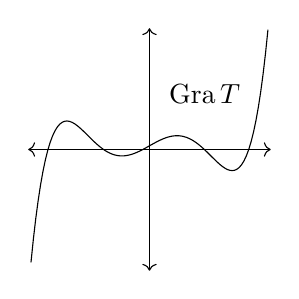
\begin{tikzpicture}[scale=.7]
\draw[domain=-2.15:2.15, variable=\x,samples=100] plot ({\x},{1/15 + (9 *(\x))/16 - (5 *(\x)^3)/6 + (\x)^5/5});
\draw (1,1) node {$\gra \opT$};
\draw [<->] (-2.2,0) -- (2.2,0);
\draw [<->] (0,-2.2) -- (0,2.2);
\end{tikzpicture}}
&
\raisebox{-.5\height}{
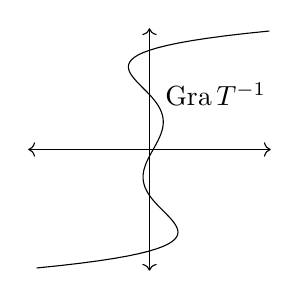
\begin{tikzpicture}[scale=.7]
\draw[domain=-2.15:2.15, variable=\x,samples=100] plot ({1/15 + (9 *(\x))/16 - (5 *(\x)^3)/6 + (\x)^5/5},{\x});

\draw (1.2,1) node {$\gra \opT^{-1}$};
\draw [<->] (-2.2,0) -- (2.2,0);
\draw [<->] (0,-2.2) -- (0,2.2);
\end{tikzpicture}}
\end{tabular}
\end{center}

\vspace{0.1in}


 $(\opT ^{-1})^{-1}=\opT $ and $\dom \opT^{-1}=\range \opT$\\
 \vspace{0.2in}

$\opT^{-1}$ is not an inverse in the usual sense since $\opT ^{-1}\opT \ne \opI$ possible.
\vspace{0.1in}

\end{frame}




\begin{frame}
\frametitle{Zero}


If $0\in \opT (x) $,  $x$ is a zero of $\opT $.

\vspace{0.2in}

Zero set of an operator $\opT $:
\[
\zer \opT  = \{x \,|\, 0\in \opT x\} = \opT ^{-1}(0)
\]

\vspace{0.2in}
Many interesting problems can be posed as finding zeros of an operator.

\end{frame}

\begin{frame}
\frametitle{Subdifferential}
When $f$ is convex:
\begin{itemize}
\item
$\partial f$ is a set-valued operator
\item
%We can start to see how this framework is useful in convex optimization by noting
$\argmin f = \zer \partial f$
\item
when $f$ is differentiable, write $\nabla f$ instead of $\partial f$
\end{itemize}
\end{frame}

\begin{frame}
\frametitle{Subdifferential of conjugate}
When $f$ is CCP,
\[
    (\partial f)^{-1}=\partial f^*
\]

\vspace{0.2in}

\textbf{Proof.}
\begin{align*}
u \in \partial f(x)
\quad& \Leftrightarrow  \quad
0\in \partial f(x)-u\\
%&\Leftrightarrow &
%f(x) \geq f(v) + u^\intercal(x-v)~\mbox{for all}~ x\\
%&\Leftrightarrow &
%f(x)-u^\intercal x \geq f(v) -u^\intercal v~\mbox{for all}~ x\\
&\Leftrightarrow \quad
x \in \argmin_ z\left\{f(z)-u^\intercal z\right\}\\
&\Leftrightarrow \quad
-f(x)+u^\intercal x =f^*(u)\\
&\Leftrightarrow \quad
f(x)+f^*(u)=u^\intercal x\\
&\Leftrightarrow \quad
f^{**}(x)+f^*(u)=u^\intercal x\\
&\Leftrightarrow \quad
x \in \partial f^* (u)
\end{align*}
The last step takes the whole argument backwards.
\qed
\end{frame}

\begin{frame}[label=subdiff-conj]
\frametitle{Subdifferential of conjugate}

$g(y)=f^*(A^\intercal y)$,
where $f$ is CCP and $ \cR(A^\intercal)\cap \relint\dom f^*\ne \emptyset$,
\begin{align*}
u\in \partial g(y)
&\quad\Leftrightarrow\quad
u\in A \partial f^*(A^\intercal y)\nonumber\\
&\quad\Leftrightarrow\quad
u= A x,\,x\in \partial f^*(A^\intercal y)\nonumber\\
&\quad\Leftrightarrow\quad
u= A x,\,\partial f(x)\ni  A^\intercal y
\label{eq:subdiff-conj}
\\
&\quad\Leftrightarrow\quad
u= A x,\,0\in \partial f(x)-  A^\intercal y\nonumber\\
&\quad\Leftrightarrow\quad
u= A x,\,x\in \argmin_z\left\{
f(z)-\langle y, Az\rangle
\right\}\nonumber
\end{align*}

\vspace{0.2in}
Find element of $\partial g$ by solving a minimization problem.
\end{frame}


\section{Monotone operators}
\begin{frame}
\frametitle{Monotone operators}
$\opT $ is monotone if
\[
\langle u-v,x-y\rangle \geq 0
\qquad\forall\,
(x,u),~(y,v) \in \opT .
\]
\vspace{0.2in}

Equivalently and more concisely, $\opT$ is monotone if
\[
\langle \opT x-\opT y,x-y\rangle \geq 0
\qquad\forall\,x,y \in\reals^n.
\]
\end{frame}

\begin{frame}
\frametitle{Maximal monotone operators}

$\opT $ is maximal monotone if $\nexists$ monotone $\opS$ such that $\gra \opT \subset \gra \opS$ properly.

\vspace{0.2in}
I.e., if $\opT $ is monotone but not maximal, then $\exists$ $(x,u)\notin  \opT $ such that
$ \opT \cup\{(x,u)\}$ is monotone.

\vspace{0.2in}

Maximality is a technical but fundamental detail.
\end{frame}

\begin{frame}
\frametitle{Monotone operator example}
Heaviside step function
\[
u(x)=\left\{
\begin{array}{ll}
0&\text{ for } x\le 0\\
1&\text{ for } x> 0\\
\end{array}
\right.
\]
is monotone but not maximal.
Operator
\[
U(x)=\left\{
\begin{array}{ll}
\{0\}&\text{ for } x< 0\\
{[0,1]}
&\text{ for } x=0 \\
\{1\}&\text{ for } x> 0
\end{array}
\right.
\]
is maximal monotone.
\vspace{-0.1in}
\begin{center}
\begin{tabular}{cc}
\raisebox{-.5\height}{
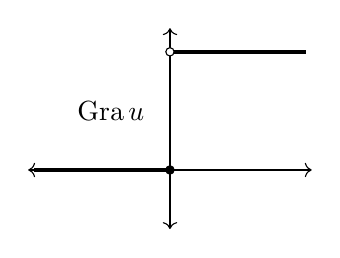
\begin{tikzpicture}[scale=1.5]
\draw [line width=1.5pt] (-1.15,0)--(0,0);
\draw [line width=1.5pt] (0,1)--(1.15,1);
\draw [<->] (-1.2,0) -- (1.2,0);
\draw [<->] (0,-.5) -- (0,1.2);
\filldraw (0,0) circle ({1pt});
\filldraw [fill=white] (0,1) circle ({1pt});
\draw (-0.5,0.5) node {$\gra u$};
\end{tikzpicture}}
&
\raisebox{-.5\height}{
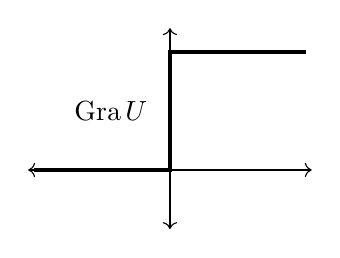
\begin{tikzpicture}[scale=1.5]
\draw [line width=1.5pt] (-1.15,0)--(0,0)-- (0,1)--(1.15,1);
\draw [<->] (-1.2,0) -- (1.2,0);
\draw [<->] (0,-.5) -- (0,1.2);
\draw (-0.5,0.5) node {$\gra U$};
\end{tikzpicture}}
\end{tabular}
\end{center}
\end{frame}

\begin{frame}[plain]
\frametitle{Monotonicity of subdifferentials}
If $f$ is convex and proper, then $\partial f$ is monotone.\\
If $f$ is CCP, then $\partial f$ is maximal monotone.
\vspace{0.2in}

\textbf{Proof of monotonicity.}
Add
\[
f(y) \geq f(x) + \langle \partial f(x),y-x\rangle, \qquad f(x) \geq f(y) + \langle \partial f(y),x-y\rangle
\]
to get
\[
\langle\partial f(x)-\partial f(y),x-y\rangle\ge 0.
\]
\qed
\vspace{0.2in}


Maximality proved later in \S10.

\vspace{0.2in}


\[
\text{[subdiff.\ CCP]}\subset \text{[maximal monotone]}
\]
strict inclusion
\end{frame}


\begin{frame}
\frametitle{Stronger monotonicity properties}
$\opA:\reals^n\rightrightarrows\reals^n$ is $\mu$-strongly monotone or $\mu$-coercive
if $\mu>0$ and
\[
\langle u-v, x-y\rangle \geq \mu \|x-y\|^2
\qquad \forall\, (x,u),(y,v)\in \opA.
\]
$\opA $ is strongly monotone if it is $\mu$-strongly monotone for some $\mu \in(0,\infty)$.

\vspace{0.2in}

$\opA $ is $\beta$-cocoercive or $\beta$-inverse strongly monotone
if $\beta>0$
%\[
%\langle \opA x-\opA y, x-y\rangle \geq \beta \|\opA x-\opA y\|^2
%\qquad \forall\, x,y\in\reals^n.
%\]
\[
\langle u-v, x-y\rangle \geq \beta \|u-v\|^2
\qquad \forall\, (x,u),(y,v)\in \opA.
\]
We say $\opA $ is cocoercive if it is $\beta$-cocoercive for some  $\beta\in(0,\infty)$.

\vspace{0.2in}
Cocoercivity and strong monotonicity are dual:\\

[$\opA $ is $\beta$-cocoercive] $\Leftrightarrow$ [$\opA ^{-1}$ is $\beta$-strongly monotone] \\

\vspace{0.2in}
Strongly monotone and cocoercive operators are monotone.
\end{frame}

\begin{frame}[plain]
\frametitle{Stronger monotonicity properties}
When $\opA $ is $\beta$-cocoercive, Cauchy-Schwartz tells us
\[
(1/\beta)\|x-y\|\geq  \|\opA x-\opA y\|\qquad \forall\, x,y\in\reals^n.
\]
i.e., $\opA $ is $(1/\beta)$-Lipschitz. Cocoercive operators are single-valued.



\vspace{0.2in}
Converse is not true. %A Lipschitz operator is not necessarily cocoercive.
\[
\opA (x_1,x_2)=\begin{bmatrix}
0&1\\
-1&0
\end{bmatrix}
\begin{bmatrix}
x_1\\x_2
\end{bmatrix}=
\begin{bmatrix}
x_2\\-x_1
\end{bmatrix}
\]
is maximal monotone and Lipschitz, but not cocoercive since $\langle \opA x-\opA y, x-y\rangle = 0$.


\vspace{0.2in}
More concisely express $\mu$-strong monotonicity as
\[
\langle \opA x-\opA y, x-y\rangle \geq \mu \|x-y\|^2
\qquad \forall\, x,y\in\reals^n,
\]
and, when $\opA$ is a priori known or assumed to be single-valued, express $\beta$-cocoercivity as
\[
\langle \opA x-\opA y, x-y\rangle \geq \beta \|\opA x-\opA y\|^2
\qquad \forall\, x,y\in\reals^n.
\]

\end{frame}


\begin{frame}
\frametitle{Stronger monotonicity properties: Maximality}
$\opA $ is maximal $\mu$-s.m.\ if $\nexists$ $\mu$-s.m.\ $\opB$ such that $\gra \opA \subset \gra \opB$ properly.
%If a maximal monotone operator is $\mu$-strongly monotone, then it is maximal $\mu$-strongly monotone.

$\opA $ is maximal $\beta$-coco.\ if $\nexists$ $\beta$-coco.\ $\opB$ such that $\gra \opA \subset \gra \opB$ properly.

\vspace{0.2in}


[Maximal coco.] and [maximal s.m.] are dual:

[$\opA $ is maximal $\beta$-coco.] $\Leftrightarrow$ [$\opA ^{-1}$ is maximal $\beta$-s.m.].

\vspace{0.2in}
If $\opA$ cocoercive,
[$\opA$ maximal] $\Leftrightarrow$ [$\dom \opA=\reals^n$].
(We prove this in \S10.)

Therefore,
``$\opA\colon\reals^n\rightarrow \reals^n$ is $\beta$-cocoercive''
implicitly asserts $\dom \opA=\reals^n$ and maximality of $\opA$.
\end{frame}


\begin{frame}
\frametitle{Stronger monotonicity properties: CCP functions}

Assume $f$ is CCP. Then
\begin{itemize}
\item

[$f$ is $\mu$-strongly convex] $\Leftrightarrow$  [$\partial f$ is $\mu$-strongly monotone]
\item

[$f$ is $L$-smooth] $\Leftrightarrow$ [$\partial f$ is $L$-Lipschitz] $\Leftrightarrow$ [$\partial f$ is $(1/L)$-cocoercive]
\item

[$f$ is $\mu$-strongly convex] $\Leftrightarrow$ [$f^*$ is $(1/\mu)$-smooth]
\end{itemize}
%\item
%Since $\partial f$ is $\mu$-strongly monotone if and only if $(\partial f)^{-1}=\partial f^*$ is $(1/\mu)$-cocoercive,
\vspace{0.2in}


\vspace{0.2in}
For $\partial f$, Lipschitz $= $ cocoercive.\\
For monotone operators, Lipschitz $\ne $ cocoercive.

\end{frame}


\begin{frame}[plain]
\frametitle{Stronger monotonicity properties examples}
Operator on $\reals$ is monotone if its graph is a nondecreasing curve in $\reals^2$.
Vertical portions, then multi-valued.
Continuous with no end points, then maximal.
Slope $\ge$ $\mu$, then $\mu$-strongly monotone.
Slope $\le $ $L$, then $L$-Lipschitz.
Lipschitz and cocoercivity coincide.
\begin{center}
\begin{tabular}{P{2.5cm}P{2.5cm}P{2.5cm}}
\raisebox{-.5\height}{
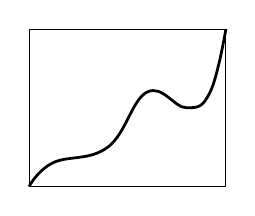
\begin{tikzpicture}[scale=1]
\draw(-1,-0.5) rectangle (1.5,1.5);
\draw[line width=1pt] plot[smooth, tension=.7] coordinates {(-1,-0.5) (-0.7,-0.2) (0,0) (0.5,0.7) (1,0.5) (1.3,0.7) (1.5,1.5)};
%\draw (0,-1) node [text width=3cm]{Not monotone};
\end{tikzpicture}}
&
\raisebox{-.5\height}{
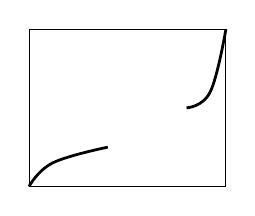
\begin{tikzpicture}[scale=1]
\draw(-1,-0.5) rectangle (1.5,1.5);
\draw[line width=1pt]  plot[smooth, tension=.7] coordinates {(-1,-0.5) (-0.7,-0.2) (0,0)};
\draw[line width=1pt]  plot[smooth, tension=.7] coordinates {(1,0.5) (1.3,0.7) (1.5,1.5)};
%\draw (0,-1) node [text width=3cm]{Monotone but not maximal};
\end{tikzpicture}}&
\raisebox{-.5\height}{
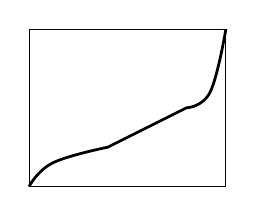
\begin{tikzpicture}[scale=1]
\draw(-1,-0.5) rectangle (1.5,1.5);
\draw[line width=1pt]  plot[smooth, tension=.7] coordinates {(-1,-0.5) (-0.7,-0.2) (0,0)}--plot[smooth, tension=.7] coordinates {(1,0.5) (1.3,0.7) (1.5,1.5)};
%\draw (0,-1) node [text width=3cm]{Maximal monotone and single-valued};
\end{tikzpicture}}\\
Not monotone & Monotone but not maximal & Maximal monotone and single-valued\\
%\vspace{0.01in}\\
\raisebox{-.5\height}{
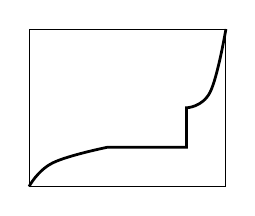
\begin{tikzpicture}[scale=1]
\draw(-1,-0.5) rectangle (1.5,1.5);
\draw[line width=1pt]  plot[smooth, tension=.7] coordinates {(-1,-0.5) (-0.7,-0.2) (0,0)} -- (1,0) -- (1,0.5) -- plot[smooth, tension=.7] coordinates {(1,0.5) (1.3,0.7) (1.5,1.5)};
%\draw (0,-1) node [text width=3cm]{Maximal monotone and multi-valued};
\end{tikzpicture}}
&
\raisebox{-.5\height}{
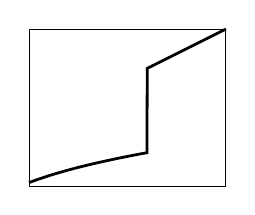
\begin{tikzpicture}[scale=1]
\draw(1,-0.5) rectangle (3.5,1.5);
\draw[line width=1pt,domain=1:2.5, variable=\x,samples=100] plot ({\x},{\x/20+ln(\x)/3-0.5})--(2.5,1)--(3.5,1.5);
%\draw (0,-1) node [text width=3cm]{Strongly monotone but not Lipschitz};
\end{tikzpicture}}
&
\raisebox{-.5\height}{
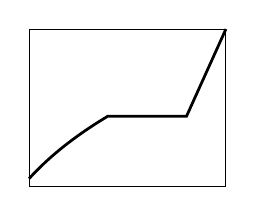
\begin{tikzpicture}[scale=1]
\draw(1,-0.5) rectangle (3.5,1.5);
\draw[line width=1pt,domain=1:2, variable=\x,samples=100] plot ({\x},{\x/10+ln(\x)-0.5})--(3,0.393147)--(3.5,1.5);
%\draw (0,-1) node[text width=3cm] {Lipschitz but not strongly monotone};
\end{tikzpicture}}\\
Maximal monotone and multi-valued&Strongly monotone but not Lipschitz&Lipschitz but not strongly monotone
\end{tabular}
\end{center}
\end{frame}




\begin{frame}
\frametitle{Operations preserving monotonicity}
\begin{itemize}
\item
 $\opT $ (maximal) monotone, then $\opS (x)=y+\alpha \opT(x+z)$ (maximal) monotone for any $\alpha>0$ and $y,z\in \reals^n$.
\item
$\opT $ (maximal) monotone, then $\opT ^{-1}$ (maximal) monotone.
\item
$\opT $ and $\opS$ monotone, $\opT +\opS $ monotone.
\item
$\opT $ and $\opS $ maximal monotone and $\dom \opT \cap\intr\dom \opS \ne \emptyset$, then $\opT +\opS $ maximal monotone.
\item
$\opT \colon\reals^n\rightrightarrows \reals^n$ monotone and $M \in \reals^{n \times m}$, then $M^\intercal\opT M$ monotone.
\item
$\opT $ maximal and $ \mathcal{R}(M)\cap \intr\dom \opT \ne \emptyset$, then $M^\intercal\opT M$ maximal.
\end{itemize}

\vspace{0.2in}

Proofs of maximality in \S10.
\end{frame}





\begin{frame}
\frametitle{Operations preserving monotonicity: Concatenation}
If $\opR \colon\reals^n\rightrightarrows \reals^n$ and $\opS \colon\reals^m\rightrightarrows \reals^m$,
then  $\opT \colon\reals^{n+m}\rightrightarrows\reals^{n+m}$
\[
\opT (x,y)=\{
(u,v)\,|\,
u\in \opR x,\,v\in \opS y
\}
\]
the concatenation of $\opR$ and $\opS$,
is (maximal) monotone if $\opR $ and $\opS $ are.
Use notation
\[
\opT =\begin{bmatrix}
\opR \\\opS
\end{bmatrix},
\qquad
\opT (x,y)=
\begin{bmatrix}
\opR x\\\opS y
\end{bmatrix}.
\]

\end{frame}



\begin{frame}
\frametitle{Operations preserving stronger monotonicity properties}
$\opT $ is $\mu$-s.m., then $\alpha\opT$ is $(\alpha \mu)$-s.m.\ for $\alpha >0$.
\vspace{0.2in}


$\opT $ is $\mu$-s.m.\ and $\opS $ monotone, then
$\opT +\opS $ is $\mu$-s.m.
\vspace{0.2in}

$\opT \colon\reals^n\rightrightarrows\reals^n$ is $\mu$-s.m., and $M\in \reals^{n\times m}$ has rank $m$, then $M^\intercal\opT  M$ is
$(\mu\sigma^2_\mathrm{min}(M))$-s.m.
\vspace{0.2in}

$\opT  \colon\reals^n\rightarrow\reals^n$ is $L$-Lipschitz and $M\in \reals^{n\times m}$, then $M^\intercal\opT  M$ is  $(L \sigma_\mathrm{max}^2(M))$-Lipschitz.

\end{frame}


\begin{frame}
%\begin{example}[Affine functions]
\frametitle{Example: Affine operators}
Affine operator $\opT (x) =Ax+b$:
\begin{itemize}
\item

[$\opT$ maximal monotone] $\Leftrightarrow$ [$A+A^\intercal \succeq 0$]
\item

[$\opT=\nabla f$ for CCP $f$] $\Leftrightarrow$ [$A=A^\intercal$ and $A\succeq 0$]
\item
$\opT$ is $\lambda_\mathrm{min}(A+A^\intercal)/2$-strongly monotone if $\lambda_\mathrm{min}(A+A^\intercal)>0$ \\
and $\sigma_\mathrm{max}(A)$-Lipschitz.
\end{itemize}
\end{frame}


\begin{frame}
\frametitle{Example: Continuous operators}
$\opT\colon\reals^n\rightrightarrows \reals^n$ is continuous if\\
$\dom \opT=\reals^n$, $\opT$ is single-valued, and $\opT$ is  continuous as a function.
\vspace{0.2in}


A continuous monotone operator $\opT \colon\reals^n\rightarrow\reals^n$ is maximal.
\vspace{0.2in}

Maximality is only in question with discontinuous or set-valued operators.
\end{frame}


\begin{frame}
\frametitle{Example: Differentiable operators}
We say an operator is differentiable if it is continuous and differentiable.

\vspace{0.2in}
For differentiable $\opT \colon \reals^n \rightarrow \reals^n$,
\begin{itemize}
\item

[$\opT$ monotone] $\Leftrightarrow$ [$D\opT (x)+D\opT (x)^\intercal \succeq 0,\,\forall x$]

\item

[$\opT$ $\mu$-s.m.]  $\Leftrightarrow$ [$D\opT (x)+D\opT (x)^\intercal \succeq 2\mu I,\,\forall x$]
\item

[$\opT$ $L$-Lipschitz] $\Leftrightarrow$ [$\sigma_\mathrm{max}(D\opT (x))\le L,\,\forall x$]
\end{itemize}

\vspace{0.2in}


Continuously differentiable monotone $\opT $,

[$\opT=\nabla f$ for CCP $f$] $\Leftrightarrow$ [$D\opT (x)$ symmetric $\forall x$]\\
(When $n=3$, this is $\nabla\times\opT=0$ condition of electromagnetic potentials.)
\end{frame}


\begin{frame}
\frametitle{Example: Saddle subdifferential}
For convex-concave $\lagrange\colon\reals^n \times \reals^m \to \reals\cup\{\pm \infty\}$,\\
saddle subdifferential operator
$\partial \lagrange\colon\reals^n \times \reals^m\rightrightarrows\reals^n \times \reals^m$:
\[\partial \lagrange(x,u) =
\left[ \begin{array}{c}  \partial_x \lagrange(x,u) \\ \partial_u (-\lagrange(x,u))
\end{array}\right]
\]
\vspace{0.2in}

$\zer\partial \lagrange$ is the set of saddle points of $\lagrange$, i.e.,\\

[$0\in \partial \lagrange(x^\star,u^\star)$] $\Leftrightarrow$ [$(x^\star,u^\star)$ is a saddle point of $\lagrange$]

\vspace{0.2in}

For most well-behaved (``closed proper'') convex-concave saddle functions, their saddle subdifferentials are maximal monotone.\\
We avoid this notion and instead verify the maximality of saddle subdifferentials on a case-by-case basis.

\end{frame}


\begin{frame}
\frametitle{Example: KKT operator}
Consider
\[
\begin{array}{ll}
\underset{x}{\mbox{minimize}}&f_0(x)\\
\mbox{subject to}&f_i(x)\le 0,\quad i=1,\ldots,m\\
&h_i(x)=0,\quad i=1,\ldots,p,
\end{array}
\]
$f_0,\dots,f_m$ are CCP and $h_1,\dots,h_p$ are affine.
Lagrangian
\[
\lagrange(x, \lambda,\nu) =f_0(x) + \sum_{i=1}^m \lambda_i f_i(x)+\sum^p_{i=1}\nu_ih_i(x)-\delta_{\reals_+^m}(\lambda)
\]
is convex-concave. Consider the Karush--Kuhn--Tucker (KKT) operator
\[
\opT (x, \lambda,\nu) = \begin{bmatrix} \partial_x \lagrange(x, \lambda,\nu) \\ -\opF(x)+\opN_{{\reals_+^m}}(\lambda)\\-\opH(x) \end{bmatrix},
\]
where
\[
\opF(x) =  \begin{bmatrix}f_1(x) \\ \vdots \\ f_m(x)\end{bmatrix},
\qquad
\opH(x) =  \begin{bmatrix} h_1(x) \\ \vdots \\ h_p(x) \end{bmatrix}.
\]
\end{frame}



\begin{frame}
\frametitle{Example: KKT operator}
\[
\opT (x, \lambda,\nu) = \begin{bmatrix} \partial_x \lagrange(x, \lambda,\nu) \\ -\opF(x)+\opN_{{\reals_+^m}}(\lambda)\\-\opH(x) \end{bmatrix}
=
\begin{bmatrix} \partial_x \lagrange(x, \lambda,\nu) \\
\partial_\lambda(-\lagrange(x, \lambda,\nu))\\
\partial_\nu(-\lagrange(x, \lambda,\nu))
 \end{bmatrix}
\]

\vspace{0.2in}
$\opT $ is a special case of the saddle subdifferential, so monotone.

\vspace{0.2in}


Arguments based on total duality tell us:\\

[$0\in \opT (x^\star,\lambda^\star,\nu^\star)$]
$\Leftrightarrow$
[$x^\star$ primal sol.,
$(\lambda^\star,\nu^\star)$ dual sol., strong duality]
\end{frame}

\begin{frame}
\frametitle{Monotone inclusion problem}
Monotone inclusion problem:
\[
\begin{array}{ll}
\underset{x\in \reals^n}{\mbox{find}}&0\in \opA x,
\end{array}
\]
where $\opA$ is monotone.

\vspace{0.2in}
Many interesting problems can be formulated this way.
\end{frame}



\section{Nonexpansive and averaged operators}
\begin{frame}
\frametitle{Nonexpansive and contractive operators}
$\opT $ is nonexpansive if
\[
\|\opT x-\opT y\|\le \|x-y\|
\qquad\forall\,x,y\in \dom \opT,
\]
i.e., $1$-Lipschitz.
$\opT $ is a contraction if $L$-Lipschitz with $L<1$.

\vspace{0.2in}
Mapping a pair of points by a contraction reduces their distance; mapping by a nonexpansive operator does not increase their distance.

\vspace{0.2in}
Properties:
\begin{itemize}
\item If $\opT $ and $\opS $ nonexpansive, then $\opT \opS $ nonexpansive.
\item If $\opT $ or $\opS $ furthermore contractive, then $\opT \opS $ contractive.
\item If $\opT $ and $\opS $ nonexpansive, then $\theta \opT  + (1-\theta)  \opS $ with $\theta \in [0,1]$ nonexpansive.
\item If $\opT $ is furthermore contractive and $\theta\in(0,1]$, then $\theta \opT  + (1-\theta)  \opS $  contractive.
\end{itemize}
\end{frame}


\begin{frame}
\frametitle{Averaged operators}
For $\theta\in (0,1)$, $\opT $ is $\theta$-averaged if $\opT =(1-\theta)\opI+\theta \opS $ for nonexpansive $\opS $.
%where the implicitly defined $\opR $ is nonexpansive.
Operator is averaged if $\theta$-averaged for some $\theta\in(0,1)$.
Operator is firmly nonexpansive if $(1/2)$-averaged.

\vspace{0.2in}

$\opT $ and $\opS $ are averaged, composition $\opT \opS $ is averaged.
(Proof later in \S13.)

\vspace{0.2in}

Averagedness is the basis for convergence of many splitting methods.
\end{frame}


\begin{frame}
\frametitle{Averaged operators}

    \begin{center}
    \begin{tabular}{ccccc}
\raisebox{-.5\height}{
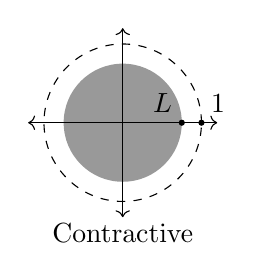
\begin{tikzpicture}[scale=1.0]
%\draw (-0.85,0.5) node {$\cG(\cN_\theta)=$};
\fill[fill=medgrey] (0,0) circle (0.75);
\draw[dashed] (0,0) circle (1);
\draw [<->] (-1.2,0) -- (1.2,0);
\draw [<->] (0,-1.2) -- (0,1.2);
\draw (1,0) node [above right] {$1$};
%\draw (-0.75,0) node [above left] {$-L$};
\filldraw (1,0) circle ({0.6*1.5/1.0pt});
\draw (0.75,0) node [above left] {$L$};
\filldraw (0.75,0) circle ({0.6*1.5/1.0pt});
\draw (0,-1.4) node  {Contractive};
\end{tikzpicture}}
&
$\subset$
&
\raisebox{-.5\height}{
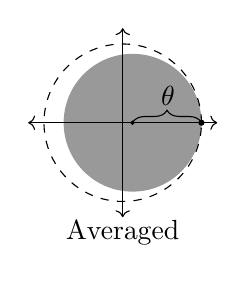
\begin{tikzpicture}[scale=1.0]
%\draw (-0.85,0.5) node {$\cG(\cN_\theta)=$};
\fill[fill=medgrey] (0.125,0) circle (0.875);
\draw[dashed] (0,0) circle (1);
\draw [<->] (-1.2,0) -- (1.2,0);
\draw [<->] (0,-1.2) -- (0,1.2);
\filldraw (.125,0) circle ({0.6*1.5/1.5pt});
\draw (0.575,0.1) node [above] {$\theta$};
%\draw (1,0) node [above right] {$1$};
\filldraw (1,0) circle ({0.6*1.5/1.0pt});
\draw [decorate,decoration={brace,amplitude=4.5pt}] (0.125,0) -- (1,0) ;
\draw (0,-1.4) node  {Averaged};
\end{tikzpicture}}
&
$\subset$&
\raisebox{-.5\height}{
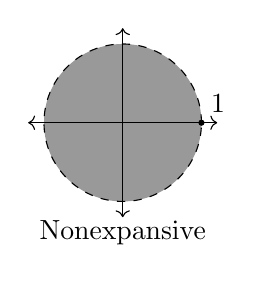
\begin{tikzpicture}[scale=1.0]
%\draw (-1.1,0.5) node {$\cG(\cL_L)=$};
\fill[fill=medgrey] (0,0) circle (1);
\draw[dashed] (0,0) circle (1);
%\draw[line width=1.0pt] (0,0) circle (0.75);
\draw [<->] (-1.2,0) -- (1.2,0);
\draw [<->] (0,-1.2) -- (0,1.2);
\draw (1,0) node [above right] {$1$};
%\draw (-0.75,0) node [above left] {$-L$};
\filldraw (1,0) circle ({0.6*1.5/1.0pt});
%\filldraw (-.75,0) circle ({0.6*1.5/1.0pt});
\draw (0,-1.4) node  {Nonexpansive};
\end{tikzpicture}}
\end{tabular}
\end{center}

\vspace{0.2in}
    Illustration of classes of contractive, averaged, and nonexpansive operators.
    The figure illustrates the relationship
     contractive $\subset$ averaged $\subset$ nonexpansive.
    The precise meaning of these figures will be defined in \S13.
\end{frame}


\section{Fixed-point iteration}

\begin{frame}
\frametitle{Fixed points}
$x$ is a fixed point of $\opT $ if $x=\opT x$.
\[
\fix \opT =
\{ x \mid x=\opT x \} = (\opI-\opT )^{-1}(0)
\]


\vspace{0.2in}
 $\fix \opT $ can contain nothing (e.g.\ $\opT x=x+1$)
or many points (e.g.\ $\opT x=|x|$).
\end{frame}

\begin{frame}
\frametitle{Fixed points}

When $\opT \colon\reals^n\rightarrow \reals^n$ is nonexpansive, $\fix \opT$ is closed and convex.

 \vspace{0.2in}

\textbf{Proof.}
 $\fix \opT $ is closed since $\opT -\opI$ is continuous.

Suppose $x,~y\in \fix \opT $, $\theta \in [0,1]$, and $z=\theta x+ (1-\theta) y  $.
Since $\opT $ is nonexpansive,
\[
\|\opT z-x\| \leq \| z-x \| = (1-\theta) \| y-x \|,
\]
Similarly,
\[
\| \opT z-y\| \leq \theta \| y-x \|.
\]
So the triangle inequality
\[
\|x-y\| \leq \|\opT z-x\| + \|\opT z-y\|
\]
holds with equality and $\opT z$ is on the line segment between
$x$ and $y$.  From $\|\opT z-y\|=\theta \|y-x\|$,
we conclude $\opT z=\theta x+ (1-\theta)y=z$. \qed
\end{frame}



\begin{frame}
\frametitle{Fixed-point iteration}
%Recall that $x$ is a fixed point of $T\colon\reals^n\rightarrow \reals^n$ if $x=Tx$.
The fixed-point iteration (FPI) is
\[
x^{k+1}=\opT x^k
\]
for $k=0,1,\dots$, where $x^0\in \reals^n$ is some starting point
and $\opT \colon\reals^n\rightarrow\reals^n$.

\vspace{0.2in}
The FPI is used to find a fixed point of $\opT $.
Clearly, the algorithm stays at a fixed point if it starts at a fixed point.


\vspace{0.2in}
Two steps of using FPI:
(i)  find a suitable  operator whose fixed points are solutions to a monotone inclusion problem of interest.
(ii) show that the iteration converges to a fixed point.

\vspace{0.2in}

In general, FPI need not converge.
We provide two guarantees.
\end{frame}


\begin{frame}
\frametitle{FPI with contractive operators}
If $\opT \colon\reals^n \rightarrow \reals^n$ is a contraction with $L<1$, then FPI is a contraction mapping algorithm.
For $x^\star\in \fix \opT $,
\[
\|x^{k}-x^\star\|
\le
L\|x^{k-1}-x^\star\|
\le\dots
\le
L^k\|x^{0}-x^\star\|.
\]
Basis of classic Banach fixed-point theorem.
When $\opT $ is a contraction, convergence is simple.
\vspace{0.2in}



In many optimization setups, however, a contraction is too much to ask for.
We need convergence under weaker assumptions.
\end{frame}


\begin{frame}
\frametitle{FPI with averaged operators}
If $\opT \colon\reals^n\rightarrow\reals^n$ is averaged, FPI is called an averaged or the Krasnosel'ski\u{\i}--Mann iteration.
\begin{theorem}
Assume $\opT \colon\reals^n\rightarrow\reals^n$ is $\theta$-averaged with $\theta\in(0,1)$
and $\fix \opT \ne \emptyset$. Then
$x^{k+1}=\opT x^k$ with any starting point $x^0\in \reals^n$
converges to one fixed point, i.e.,
\[
x^k\rightarrow x^\star
\]
 for some $x^\star\in \fix \opT $.
The quantities
$ \dist(x^{k},\fix \opT )$,
$\|x^{k+1}-x^k\|$,
and
$\|x^{k}-x^\star\|$  for any $x^\star\in \fix \opT $ are monotonically nonincreasing with $k$.
Finally, we have
\[
\dist(x^{k},\fix \opT )\rightarrow 0
\]
and
\[
\|x^{k+1}-x^k\|^2 \leq \frac{ \theta}
{(k+1) (1-\theta)}\dist^2(x^0,\fix \opT ).
\]
\vspace{-0.1in}
\end{theorem}
\end{frame}


\begin{frame}[plain]
\frametitle{Discussion of Theorem 1}
When $\opT $ is nonexpansive but not averaged, we can use $(1-\theta)\opI+\theta \opT $ with $\theta\in (0,1)$ since $\fix \opT  = \fix ((1-\theta)\opI+\theta \opT) $.

\vspace{0.2in}
For example, $\opT \colon\reals^2\rightarrow\reals^2$
\[
\opT x=\begin{bmatrix}
-0.5&0\\
0&1
\end{bmatrix}x
\]
is $(3/4)$-averaged with $\fix \opT  = \{(0,z)\,|\,z\in \reals\}$.
%\vspace{-0.1in}
\begin{center}
\raisebox{-.5\height}{
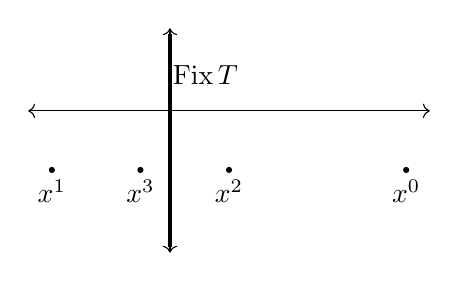
\begin{tikzpicture}[scale=1.5]
%\draw [line width=1.5pt] (-1.15,0)--(0,0);
\draw [line width=1.5pt] (0,.65)--(0,-1.15);
\draw [<->] (-1.2,0) -- (2.2,0);
\draw [<->] (0,-1.2) -- (0,0.7);
\filldraw (2,-0.5) circle ({0.6*1.5/1.5pt});
\filldraw (-1,-0.5) circle ({0.6*1.5/1.5pt});
\filldraw (0.5,-0.5) circle ({0.6*1.5/1.5pt});
\filldraw (-0.25,-0.5) circle ({0.6*1.5/1.5pt});
\draw (0.3,0.3) node {$\fix \opT$};
% \draw (1.8,-0.5) node[above right] {$(x_0,y_0)$};
% \draw (-.6,-0.5) node[below left] {$\opT(x_0,y_0)$};
% \draw (0.3,-0.5) node[below right] {$\opT \opT(x_0,y_0)$};
% \draw (-0.,-0.5) node[above left] {$\opT \opT \opT(x_0,y_0)$};
\draw (2,-0.5) node[below] {$x^0$};
\draw (-1,-0.5) node[below] {$x^1$};
\draw (0.5,-0.5) node[below] {$x^2$};
\draw (-0.25,-0.5) node[below] {$x^3$};
\end{tikzpicture}}
\end{center}
%\vspace{-0.1in}
FPI with respect to $\opT $ converges to one fixed point, which depends on the staring put $x^0$.
\end{frame}


\begin{frame}
\frametitle{Proof outline of Theorem 1}
Assume \emph{nonnegative} sequences
$V^0,V^1,\dots$
and
$S^0,S^1,\dots$ satisfy
\[
V^{k+1}\le V^k-S^k.
\]
Consequences: (i) $V^k$ is monotonically nonincreasing (although $V^k\nrightarrow 0$ possible)
(ii) $S^k\rightarrow 0$.
To see why, sum both sides from $0$ to $k$ to get
\[
\sum^k_{i=0}S^i \le V^0-V^{k+1}\le V^0.
\]
Taking $k\rightarrow\infty$ gives us
\[
\sum^\infty_{i=0}S^i \le V^0<\infty.
\]
$S^0,S^1,\dots$ is summable. By summability, $S^k\rightarrow 0$.
$V^k$ is a the Lyapunov function and $S^k$ the summable term. This is the summability argument.
\end{frame}

\begin{frame}
\frametitle{Proof of Theorem 1}
\textbf{Stage 1.}
Note the identity
\[
\| (1-\theta) x + \theta y \|^2 = (1-\theta) \|x\|^2 +
\theta \|y\|^2 - \theta(1-\theta) \|x-y\|^2.
\]
%which holds for any $\theta \in \reals$, $x,y \in \reals^n$.
%Verifying the identity is a matter of expanding both
%sides.
% For $\theta \in (0,1)$, we can view \eqref{e-quad-ident} as a strengthening of Jensen's inequality.

$\opT =(1-\theta)\opI+\theta \opS$, where $\opS$ is N.E.
Then
\[
x^{k+1}=\opT x^k=(1-\theta)x^k+\theta \opS x^k.
\]
For any $x^\star \in \fix \opT $,
\begin{align}
\|x^{k+1}& - x^\star\|^2 \nonumber\\&=
(1-\theta) \|x^k - x^\star\|^2 +
\theta \|\opS (x^k) - x^\star \|^2 - \theta(1-\theta)
\|\opS (x^k)-x^k\|^2\nonumber\\
&\leq
(1-\theta) \|x^k - x^\star\|^2 +
\theta \|x^k - x^\star \|^2 - \theta(1-\theta)
\|\opS (x^k)-x^k\|^2\nonumber\\
&=
\underbrace{\|x^k - x^\star\|^2}_{=V^k} -
\underbrace{\theta(1-\theta) \|\opS (x^k)-x^k\|^2}_{=S^k}.
\label{e-point-fejer}
\end{align}
\end{frame}

\begin{frame}
\frametitle{Proof of Theorem 1}
Now establish the monotonic decreases.
Core inequality \eqref{e-point-fejer} tells us
\[
\|x^{k+1}-x^\star\|\le \|x^{k}-x^\star\|.
\]
Minimize both sides with respect to $x^\star\in \fix \opT $:
\[
\dist(x^{k+1},\fix \opT )\le  \dist(x^k,\fix \opT ).
\]
This is called Fej\'er monotonicity.

\vspace{0.2in}


Fixed-point residual: $\opT (x^k)-x^k=x^{k+1}-x^k$.
We view $\|\opT (x^k)-x^k\|$ as a measure of optimality for FPI.
%the magnitude of the fixed point residual
Since $\opT $ is nonexpansive,
\[
\|x^{k+1}-x^k\|= \|\opT x^{k}-\opT x^{k-1}\|\le \|x^{k}-x^{k-1}\|.
\]
%The summability argument applied to \eqref{e-point-fejer} tells us $\|x^{k+1}-x^k\|\rightarrow 0$.
\end{frame}

\begin{frame}[plain]
\frametitle{Proof of Theorem 1}
%Using the monotonic decrease of $\|x^{k+1}-x^k\|$, we obtain a rate of convergence for $\|x^{k+1}-x^k\|\rightarrow 0$.
\vspace{0.1in}
Sum \eqref{e-point-fejer} from $0$ to $k$
\[
\|x^{k+1} - x^\star\|^2 \leq
\|x^0 - x^\star\|^2 - \frac{1-\theta}{\theta}\sum_{j=0}^k
 \|\opT x^{j}-x^j\|^2
\]
\vspace{-0.2in}

Reorganize
\[
\sum_{j=0}^k \|\opT x^{j}-x^j\|^2\leq \frac{\theta}{1-\theta}\|x^0 - x^\star\|^2 -\frac{\theta}{1-\theta}\|x^{k+1} - x^\star\|^2
\]
\vspace{-0.1in}

Monotonicity of $\|x^{k+1}-x^k\|$
\[
(k+1)\|x^{k+1}-x^k\|^2
\le \sum_{j=0}^k\|x^{j+1}-x^j\|^2\leq \frac{\theta}{1-\theta}\|x^0 - x^\star\|^2
\]
\vspace{-0.2in}

Conclude
\[
\|x^{k+1}-x^k\|^2 \leq \frac{ \theta}
{(k+1) (1-\theta)}\|x^0 - x^\star\|^2.
\]
Minimizing the right-hand side with respect to $x^\star\in \fix \opT $
\[
\|x^{k+1}-x^k\|^2 \leq \frac{ \theta}
{(k+1) (1-\theta)}\dist^2(x^0,\fix \opT ).
\]
\end{frame}




\begin{frame}
\frametitle{Convergence proof of Theorem 1}
\textbf{Stage 2.}
Now show $x^k\rightarrow x^\star$ for some $x^\star\in \fix \opT $ with the steps:\\
(i) $x^k$ has an accumulation point (ii) this accumulation point is a solution (iii) this is the only accumulation point.

\begin{itemize}
\item[(i)]
Consider any $\tilde{x}^\star\in \fix \opT $.
Then \eqref{e-point-fejer}
tells us that $x^0,x^1,\dots$
lie within the compact set $\{x\,|\,\|x-\tilde{x}^\star\|\le \|x^0-\tilde{x}^\star\|\}$,
and $x^0,x^1,\dots$ has an accumulation point $x^\star$.
\item[(ii)]
Accumulation point $x^\star$ satisfies $\opT (x^\star)-x^\star=0$, as $\opT (x^k)-x^k\rightarrow 0$ and $\opT -\opI$ is continuous, i.e., $x^\star\in \fix \opT $.
\item[(iii)]
Apply \eqref{e-point-fejer} to this accumulation point $x^\star\in \fix \opT $
to conclude $\|x^k-x^\star\|$ monotonically decreases to $0$,
i.e., the entire sequence converges to $x^\star$.
\end{itemize}



\qed
\end{frame}

\begin{frame}
\frametitle{Termination criterion}

$\|x^{k+1}-x^k\|<\varepsilon$ can be used as a termination criterion.\\
Specific setups may have specific and better termination criteria.

\vspace{0.2in}

We avoid the discussion of termination criterion for simplicity.
\end{frame}


\begin{frame}
\frametitle{Methods: Gradient descent}
Consider
\[
\underset{x\in \reals^n}{\mbox{minimize}}~f(x),
\]
where $f$ is CCP and differentiable.

\vspace{0.2in}
[$x\in \mathrm{argmin} f$]
$\Leftrightarrow $
[$x=(\opI -\alpha \nabla f)(x)$ for any nonzero $\alpha\in \reals$]

\vspace{0.2in}

The FPI
\[
x^{k+1}=x^k-\alpha \nabla f(x^k)
\]
is gradient method or gradient descent, and $\alpha$ is the step size.
\end{frame}

\begin{frame}
\frametitle{Methods: Gradient descent}
Assume $f$ is $L$-smooth. By cocoercivity,
\begin{align*}
&\|(\opI -(2/L)\nabla f)x-(\opI -(2/L)\nabla f)y\|^2\\
&=
\|x-y\|^2-\frac{4}{L}
\left(\langle x-y,\nabla f(x)-\nabla f(y)\rangle-
\frac{1}{L}\|\nabla f(x)-\nabla f(y)\|^2 \right)\\
&\le
\|x-y\|^2.
\end{align*}
Therefore, $\opI -\alpha\nabla f$ is
averaged for $\alpha\in(0,2/L)$ since
\[
\opI -\alpha \nabla f=
(1-\theta)\opI
+\theta(\opI -(2/L) \nabla f),
\]
where $\theta=\alpha L/2<1$.

\vspace{0.2in}

$x^k\rightarrow x^\star$ if a solution exists with rate
\[
\|\nabla f(x^k)\|^2=O(1/k),
\]
for any $\alpha\in(0,2/L)$.

\vspace{0.2in}
If $f$ is strongly convex, FPI is a contraction.
\end{frame}

\begin{frame}
\frametitle{Methods: Forward step method}
Consider
\[
\begin{array}{ll}
\underset{x\in \reals^n}{\mbox{find}}&0= \opF (x),
\end{array}
\]
where $\opF \colon\reals^n\rightarrow \reals^n$.
\vspace{0.2in}

[$x\in \zer \opF$] $\Leftrightarrow$ [$x\in \fix(\opI-\alpha \opF)$ for any nonzero $\alpha\in \reals$]

\vspace{0.2in}


The FPI
\[
x^{k+1}=x^k-\alpha \opF x^k,
\]
is the forward step method.
\vspace{0.2in}


$x^k\rightarrow x^\star$ if $\opF $ is $\beta$-cocoercive, $\alpha\in (0,2\beta)$, and $\fix \opF\ne \emptyset$.\\
Contraction for small $\alpha>0$ if $\opF $ is strongly monotone and Lipschitz.
\end{frame}


\begin{frame}
\frametitle{Methods: Dual ascent}
Consider primal-dual problem pair
\[
\begin{array}{ll}
\underset{x\in \reals^n}{\mbox{minimize}} &f(x)\\
\mbox{subject to} &Ax=b,
\end{array}
\qquad
\begin{array}{ll}
\underset{u\in\reals^m}{\mbox{maximize}}&- f^*(-A^\intercal u)-b^\intercal u
\end{array}
\]
and its associated Lagrangian
\[
\lagrange(x,u)=f(x)+\langle u,Ax-b\rangle.
\]
\vspace{0.2in}

Gradient method on $g(u)=f^*(-A^\intercal u)+b^\intercal u$, the FPI on $\opI-\alpha\nabla g$
\begin{align*}
x^{k+1}&=\argmin_x \lagrange(x,u^k)\nonumber\\
u^{k+1}&=u^k+\alpha (Ax^{k+1}-b)
\end{align*}
Uzawa method or dual ascent.
($\nabla g$ characterized in page~\ref{subdiff-conj}.)

\end{frame}

\begin{frame}
\frametitle{Methods: Dual ascent}

If $f$ is $\mu$-strongly convex, then
%, then $f^*$ is differentiable and $\nabla f^*$ is $(1/\mu)$-Lipschitz.
\[
\nabla g(u)=-A\nabla f^*(-A^\intercal u)+b
\]
is Lipschitz with parameter $\sigma_\mathrm{max}^2(A)/\mu$.
\vspace{0.2in}

If $f$ is $\mu$-strongly convex, total duality holds, and $0<\alpha<2\mu/\sigma^2_\mathrm{max}(A)$,
then $x^k\rightarrow x^\star$ and $u^k\rightarrow u^\star$.
\end{frame}

\section{Resolvents}
\begin{frame}
\frametitle{Resolvent and reflected resolvent}
Resolvent $\opA$:
\[
\opJ_{\opA}= (\opI+\opA)^{-1}
\]
Reflected resolvent of $\opA$:
\[
\opR_{\opA} = 2\opJ_{\opA}-\opI
\]
also called Cayley operator or reflection operator.\\
Often use $\opJ_{\alpha \opA}$ and $\opR_{\alpha \opA}$ with $\alpha>0$.
\vspace{0.2in}


If $\opA$ is maximal monotone,
$\opR_\opA$ is a nonexpansive (single-valued) with $\dom \opR_\opA=\reals^n$,
and
$\opJ_\opA$ is a $(1/2)$-averaged with $\dom \opJ_\opA=\reals^n$.
\end{frame}


\begin{frame}
\frametitle{Nonexpansiveness of $\opR_\opA$ and $\opJ_\opA$}
Proof of nonexpansiveness and averagedness.
\vspace{0.2in}

\textbf{Proof.}
Assume $(x,u),(y,v)\in \opJ_\opA$. Then
\[
x\in u + \opA u,\qquad
y\in v+\opA v.
\]
By monotonicity of $\opA$,
\[
\langle(x-u)-(y-v),
u-v
\rangle\ge 0
\]
and
\begin{align*}
\|(2u-x)-(2v-y)\|^2
 &= \|x-y\|^2 - 4
 \langle(x-u)-(y-v),
u-v
\rangle\\
&\le \|x-y\|^2.
\end{align*}
So $\opR_\opA$ is NE and $\opJ_\opA=(1/2)\opI+(1/2)\opR_\opA$ is $(1/2)$-averaged.
\qed
\end{frame}


\begin{frame}
\frametitle{Domain of $\opR_\opA$ and $\opJ_\opA$}

Minty surjectivity theorem: $\dom \opJ_\opA=\reals^n$ when $\opA$ is maximal monotone.
\vspace{0.2in}


This result is easy to intuitively see in 1D but is non-trivial in higher dimensions.
We prove this in  \S10.

\end{frame}

\begin{frame}
\frametitle{Zero set of a maximal monotone operator}
$\zer \opA$ is a closed convex set when $\opA$ is maximal monotone.

\vspace{0.2in}
\textbf{Proof.}
$\zer \opA=\fix \opJ_\opA $ since
\[
0\in \opA x
\quad\Leftrightarrow\quad
x\in x+\opA x
\quad\Leftrightarrow\quad
\opJ_\opA x = x.
\]
Since $\opJ_\opA$ is nonexpansive, $\fix \opJ_\opA=\zer \opA$ is a closed convex set.\qed
\vspace{0.2in}

Note that proof relies on maximality through $\dom \opJ_\opA=\reals^n$.
\end{frame}


\begin{frame}
\frametitle{Example: Monotone linear operator}
Let $\opA$ be a monotone linear operator represented by a symmetric matrix.

\vspace{0.2in}
%If $\opA$ is a symmetric matrix and $\opA$ is monotone,
Then, $\opA$ has eigenvalues in $[0,\infty)$
and $\opJ_{  \opA}=(\opI+  \opA)^{-1}$ has eigenvalues in $(0,1]$.
\[
\opR_{  \opA}=2\opJ_{  \opA}-\opI=(\opI-  \opA)(\opI+  \opA)^{-1}=(\opI+\opA)^{-1}(\opI-\opA),
\]
is the Cayley transform of $\opA$ and has eigenvalues in $(-1,1]$.
\end{frame}

\begin{frame}
\frametitle{Example: Complex number as operator on $\reals^2\cong \mathbb{C}$}
Identify $z\in \mathbb{C}$ with a linear operator from $\mathbb{C}$ to $\mathbb{C}$ defined by multiplication,
i.e.,  $z\colon x\mapsto zx$.
\vspace{0.2in}

Equip complex numbers with inner product $\langle x,y\rangle =\Re x\overline{y}$.



\vspace{-0.01in}
\begin{center}
\begin{tabular}{ccc}
\raisebox{-.5\height}{
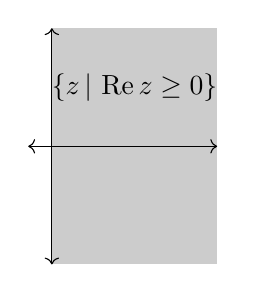
\begin{tikzpicture}[scale=1.5]
\fill [fill=lightgrey] (0,-1)--(0,1)--(1.4,1)--(1.4,-1);
\draw [<->] (-.2,0) -- (1.4,0);
\draw [<->] (0,-1) -- (0,1);
\draw (0.7,0.5) node {$\left\{z\,|\,\Re z\ge 0\right\}$};
\end{tikzpicture}}
&
\qquad\qquad\qquad
&
\raisebox{-.5\height}{
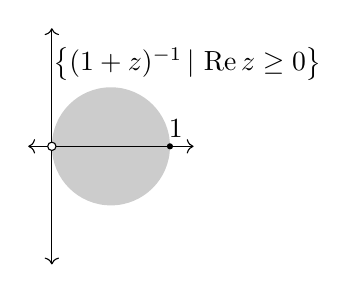
\begin{tikzpicture}[scale=1.5]
\fill[fill=lightgrey] (0.5,0) circle (0.5);
\draw [<->] (-.2,0) -- (1.2,0);
\draw [<->] (0,-1) -- (0,1);
\filldraw [fill=white] (0,0) circle ({1pt});
\draw (1.15,0.7) node {$\left\{(1+z)^{-1}\,|\,\Re z\ge 0\right\}$};
\filldraw (1,0) circle ({0.6*1.5/1.5pt});
\draw (1.05,0.15) node {$1$};
\end{tikzpicture}}
\end{tabular}
\end{center}
\vspace{0.1in}

$z\in \mathbb{C}$ is monotone if and only if $\Re z\ge 0$.
Resolvent $(1+ z)^{-1} $ for monotone $z$ is in disk with center $1/2$ and radius $1/2$ excluding origin.
\end{frame}

\begin{frame}
\frametitle{Resolvent of subdifferential}
For CCP $f$ and $\alpha>0$,
\[
\opJ_{\alpha \partial f}=\prox_{\alpha f}.
\]

\vspace{0.2in}
\textbf{Proof.}
\begin{align*}
z = (I+\alpha \partial f)^{-1}(x)
\quad&\Leftrightarrow\quad
z +\alpha \partial f(z)  \ni x\\
&\Leftrightarrow\quad
0 \in \partial_z \left(\alpha f(z) + \frac{1}{2}\|z-x\|^2\right)\\
&\Leftrightarrow\quad
z = \argmin_z
\left\{\alpha f(z) + \frac{1}{2}\|z-x\|^2\right\}\\
&\Leftrightarrow\quad
z =\prox_{\alpha f}(x)
\end{align*}
\qed
\end{frame}


\begin{frame}[label=res_subdiff_conj]
\frametitle{Resolvent of subdifferential of conjugate}
If $g(u)=f^*(A^\intercal u)$, $f$ CCP, and $ \relint\dom f^*\cap \cR(A^\intercal)\ne \emptyset$,
then
\begin{align*}
v=\prox_{\alpha g}(u)
\quad\Leftrightarrow\quad
\begin{array}{l}
x\in\argmin_x\left\{
f(x)-\langle u,Ax\rangle +\frac{\alpha}{2}\|Ax\|^2
\right\}\\
v= u-\alpha Ax.
\end{array}
% &x\in
% \argmin_x\left\{
% f(x)-\langle u,Ax\rangle +\frac{\alpha}{2}\|Ax\|^2
% \right\}\nonumber\\
% &v= u-\alpha Ax.
\end{align*}

\vspace{0.2in}

\textbf{Proof.}
\begin{align*}
v= (I+&\alpha\partial g)^{-1}(u)\\
&\quad\Leftrightarrow\quad
v+\alpha A\partial f^*(A^\intercal v)\ni u\\
&\quad\Leftrightarrow\quad
v+\alpha Ax= u,\,x\in \partial f^*(A^\intercal v)\\
&\quad\Leftrightarrow\quad
v= u-\alpha Ax,\,\partial f(x)\ni  A^\intercal v\\ %\numberthis\label{eq:prox_of_conj_comp}\\
&\quad\Leftrightarrow\quad
v= u-\alpha Ax,\,\partial f(x)\ni  A^\intercal(u-\alpha Ax)\\
%&\quad\Leftrightarrow\quad
%v= u-\alpha Ax,\,0\in \partial f(x)-  A^\intercal(u-\alpha Ax)\\
&\quad\Leftrightarrow\quad
v= u-\alpha Ax,\,x\in
\argmin_x\left\{
f(x)-\langle u,Ax\rangle +\frac{\alpha}{2}\|Ax\|^2
\right\}.
\end{align*}
\end{frame}

\begin{frame}
\frametitle{Projection is a resolvent}
If $C\subset\reals^n$ is nonempty closed convex, then
\[
\opJ_{\opN_C}=\prox_{\delta_C}=\proj_C.
\]

\vspace{0.2in}
The resolvent generalizes the projection operator in this sense.

\end{frame}
%Remember from \S\ref{c:prelim} that $\delta_C$ is the indicator function of $C$, $\opN_C$ is the normal cone operator of $C$, and $\proj_C$ is the projection onto $C$.
%These satisfy following properties:
%$\delta_C=\alpha \delta_C$ and $\opN_C=\alpha \opN_C$ for any $\alpha>0$;

\begin{frame}[label=kkt_resolvent]
\frametitle{KKT operator for linearly constrained problems}
Consider the Lagrangian
\[
\lagrange(x,u)=f(x)+\langle u,Ax-b\rangle
\]
which generates the primal problem
% of \eqref{eq:mm-lagrangian}  The saddle subdifferential $\partial \lagrange$ is the KKT operator of \eqref{eq:mm-primal},
\[
\begin{array}{ll}
\underset{x\in \reals^n}{\mbox{minimize}} &f(x)\\
\mbox{subject to} &Ax=b.
\end{array}
\]
We can compute its resolvent with
\begin{align*}
\opJ_{\alpha \partial \lagrange}(x,u )=(y,v)
\quad\Leftrightarrow\quad
\begin{array}{l}
y = \argmin_z \left\{ \lagrange_\alpha (z,u)+ \frac{1}{2\alpha}\|z-x\|^2 \right\}\\
v = u + \alpha(Ay-b),
\end{array}
\end{align*}
where $\lagrange_\alpha$ is the augmented Lagrangian
\[
\lagrange_\alpha(x,u)=f(x)+\langle u,Ax-b\rangle+\frac{\alpha}{2}\|Ax-b\|^2.
\]

\end{frame}

\begin{frame}
\frametitle{KKT operator for linearly constrained problems}
\textbf{Proof.}
For any $\alpha>0$,
\begin{align*}
(y,v)=\opJ_{\alpha \partial \lagrange}(x,u )
\quad&\Leftrightarrow\quad
\begin{bmatrix}
x\\u
\end{bmatrix}
\in
\begin{bmatrix}
y\\v
\end{bmatrix}
+
\alpha
\begin{bmatrix}
\partial f(y)+A^\intercal v\\
b-Ay
\end{bmatrix}\\
\quad&\Leftrightarrow\quad
\begin{bmatrix}
x\\u
\end{bmatrix}
\in
\alpha
\begin{bmatrix}
 \partial f(y)\\
b
\end{bmatrix}
+
\begin{bmatrix}
I&\alpha A^\intercal\\
-\alpha A &I
\end{bmatrix}
\begin{bmatrix}
y\\v
\end{bmatrix}.
\end{align*}
Left-multiply invertible matrix
\[
\begin{bmatrix}
I&-\alpha A^\intercal\\
0&I
\end{bmatrix}
\]
to get
\[
\Leftrightarrow\quad
\begin{bmatrix}
x-\alpha A^\intercal u\\u
\end{bmatrix}
\in
\alpha
\begin{bmatrix}
 \partial f(y)-\alpha A^\intercal b\\
b
\end{bmatrix}
+
\begin{bmatrix}
I+\alpha^2A^\intercal A&0\\
-\alpha A &I
\end{bmatrix}
\begin{bmatrix}
y\\v
\end{bmatrix}.
\]
First line is independent of $v$, so we can compute $y$ first and then $v$.
(This is the Gaussian elimination technique of \S3.4.)
\end{frame}

\begin{frame}
\frametitle{KKT operator for linearly constrained problems}
Reorganize to get
\begin{gather*}
0\in
  \partial f(y)
+  A^\intercal u
-\alpha A^\intercal(Ay-b)
+
(1/\alpha)(y-x)\\
v = u +\alpha (Ay-b),
\end{gather*}
and conclude
\begin{align*}
y &= \argmin_z \left\{
f(z)+\langle u,Az-b\rangle+\frac{\alpha}{2}\|Az-b\|^2+ \frac{1}{2\alpha}\|z-x\|^2 \right\}\\
v &= u + \alpha(Ay-b).
\end{align*}
\qed
\end{frame}



\begin{frame}[label=res_identities]
\frametitle{Resolvent identities}
Let $\opA$ maximal monotone and $\alpha>0$.

\vspace{0.2in}
If $\opB(x)=\opA(x)+t$,
\[
\opJ_{\alpha \opB}(u)=\opJ_{\alpha \opA}(u-\alpha t).
\]

\vspace{0.2in}

If $\opB(x)=\opA(x-t)$,
\[
\opJ_{\alpha \opB}(u)=\opJ_{\alpha \opA}(u-t)+t.
\]

\vspace{0.2in}
If $\opB(x)=-\opA(t-x)$,
\[
\opJ_{\alpha \opB}(u)=t-\opJ_{\alpha \opA}(t-u).
\]
\end{frame}




\begin{frame}
\frametitle{Inverse resolvent identity}
Inverse resolvent identity:
\[
\opJ_{\alpha^{-1} \opA}(x)+\alpha^{-1}\opJ_{\alpha \opA^{-1}}(\alpha x)=x,
\]
for maximal monotone $\opA$ and $\alpha>0$.

%This follows from
%\begin{align*}
%x-\opJ_{\alpha^{-1}\opA}x=y
%&\quad\Leftrightarrow\quad
%x\in x-y+\alpha^{-1} \opA(x-y)\\
%&\quad\Leftrightarrow\quad
%\alpha y\in \opA(x-y)\\
%&\quad\Leftrightarrow\quad
%\opA^{-1}(\alpha y)\ni x-y\\
%&\quad\Leftrightarrow\quad
%(\opI+\alpha \opA^{-1})(\alpha y)\ni \alpha x\\
%&\quad\Leftrightarrow\quad
% y=
%(1/\alpha)\opJ_{\alpha \opA^{-1}}( \alpha x).
%\end{align*}

\vspace{0.2in}
When $\alpha=1$,
\[
\opJ_{ \opA}+\opJ_{\opA^{-1}}=\opI.
\]

\vspace{0.2in}

Moreau identity: a special case, for CCP $f$
\[
\prox_{\alpha^{-1}f}(x)+\alpha^{-1}\prox_{\alpha f^*}(\alpha x)=x.
\]

\vspace{0.2in}

Consequence:
$\prox_{\alpha f}$ and $\prox_{\alpha f^*}$ require same computational cost.
% In other words, if you can compute $\prox_{\alpha f}$, then you can compute $\prox_{\alpha f^*}$, and vice versa.

\end{frame}

\begin{frame}
\frametitle{Reflected resolvent identities}
If $\opA$ is maximal monotone  and single-valued and $\alpha>0$,
\[
\opR_{\alpha \opA}=(\opI-\alpha \opA)(\opI+\alpha \opA)^{-1}.
\]
\vspace{0.2in}

\textbf{Proof.}
\begin{align*}
\opR_{\alpha \opA}&=2(\opI+\alpha \opA)^{-1}-\opI\\
&=
2(\opI+\alpha \opA)^{-1}-
(\opI+\alpha \opA)
(\opI+\alpha \opA)^{-1}\\
&=
(\opI-\alpha \opA)(\opI+\alpha \opA)^{-1}.
\end{align*}
2nd line by Exercise 2.1.
\qed
\end{frame}

\begin{frame}[label=refl-identities]
\frametitle{Reflected resolvent identities}
If $\opA$ is maximal monotone (but not necessarily single-valued)
and $\alpha> 0$,
\[
\opR_{\alpha \opA}(\opI+\alpha \opA)
=\opI-\alpha \opA.
\]

\vspace{0.2in}

\textbf{Proof.}
For $x\in \dom \opA$,
\begin{align*}
\opR_{\alpha \opA}(\opI+\alpha \opA)(x)
&=2(\opI+\alpha \opA)^{-1}(\opI+\alpha \opA)(x)
-(\opI+\alpha \opA)(x)\\
&=2\opI(x)-(\opI+\alpha \opA)(x)\\
&=(\opI-\alpha \opA)(x)
\end{align*}
2nd line by Exercise 2.1.
For $x\notin \dom \opA$, both sides are empty.
\qed
\end{frame}


\section{Proximal point method}
\begin{frame}
\frametitle{Proximal point method}
Consider
\[
\begin{array}{ll}
\underset{x\in \reals^n}{\mbox{find}}&0\in \opA x
\end{array}
\]
where $\opA$ is maximal monotone.
Equivalent to finding $x\in \fix\opJ_{\alpha \opA}$.

\vspace{0.2in}
The FPI
\[
x^{k+1} = \opJ_{\alpha \opA}(x^k)
\]
is the proximal point method (PPM) or proximal minimization.

\vspace{0.2in}
PPM converges to a solution if one exists, since $\opJ_{\alpha \opA}$ is averaged.
\end{frame}


\begin{frame}
\frametitle{Methods of multipliers}
Consider the primal-dual problem pair
% \eqref{eq:mm-primal} and \eqref{eq:mm-dual}
\[
\begin{array}{ll}
\underset{x\in \reals^n}{\mbox{minimize}} &f(x)\\
\mbox{subject to} &Ax=b,
\end{array}
\qquad
\begin{array}{ll}
\underset{u\in\reals^m}{\mbox{maximize}}&- f^*(-A^\intercal u)-b^\intercal u
\end{array}
\]
generated by the Lagrangian $\lagrange(x,u)=f(x)+\langle u,Ax-b\rangle$.\\

\vspace{0.2in}
Augmented Lagrangian:
\[
\lagrange_\alpha(x,u)=f(x)+\langle u,Ax-b\rangle+\frac{\alpha}{2}\|Ax-b\|^2.
\]
\end{frame}

\begin{frame}
\frametitle{Method of multipliers}
%\label{s-mom}
%\subsubsection{Multiplier to residual mapping.}
Assume $\cR(A^\intercal)\cap \relint \dom f^*\ne\emptyset$.
Write $g(u)=f^*(-A^\intercal u)+b^\intercal u$.

\vspace{0.2in}

The FPI $u^{k+1}=\opJ_{\alpha \partial g}(u ^k)$
\begin{align*}
x^{k+1} &\in \argmin_x \lagrange_\alpha (x,u^k)\\
u^{k+1} &= u^k+\alpha (Ax^{k+1}-b)
\end{align*}
is the method of multipliers.
($\prox_{\alpha g}$  calculation  in pages \pageref{res_subdiff_conj} and \pageref{res_identities}.)

\vspace{0.2in}

If a dual solution exists and $\alpha>0$, then $u^k\rightarrow u^\star$.
\end{frame}

\begin{frame}
\frametitle{Proximal method of multipliers}
The FPI $(x^{k+1},u^{k+1})=\opJ_{\alpha \partial \lagrange}(x^{k},u ^k)$
\begin{align*}
x^{k+1} &= \argmin_x \left\{\lagrange_{\alpha} (x,u^k)
+\frac{1}{2\alpha}\|x-x^k\|^2\right\}\\
u^{k+1} &= u^k+\alpha (Ax^{k+1}-b)
\end{align*}
is the proximal method of multipliers.
($\opJ_{\alpha \partial \lagrange}$ calculation in page \pageref{kkt_resolvent}.)
\vspace{0.2in}

If total duality holds and $\alpha>0$, then $x^k\rightarrow x^\star$ and $u^k\rightarrow u^\star$.
%where $x^\star$ and $u^\star$ are primal and dual solutions.

\end{frame}



\section{Operator splitting}

\begin{frame}
\frametitle{Operator splitting}

Operator splitting:
split a monotone inclusion problem into smaller simpler components.

\vspace{0.2in}

Specifically, transform monotone inclusion problems
 $x\in \zer(\opA+\opB)$
or $x\in \zer(\opA+\opB+\opC)$
into fixed-point equations constructed from $\opA$, $\opB$, $\opC$, and their resolvents.


\vspace{0.2in}
Unified approach: formulate optimization problem as monotone inclusion problem, apply a splitting scheme, and use the FPI.
\end{frame}


\begin{frame}
\frametitle{Forward-backward splitting}
Consider
\[
\begin{array}{ll}
\underset{x\in \reals^n}{\mbox{find}}&0\in (\opA+\opB ),
\end{array}
\]
where $\opA$ and $\opB $ maximal monotone, $\opA$ single-valued.
\vspace{0.2in}

For $\alpha>0$,
\begin{align*}
0\in (\opA+\opB )x
\quad&\Leftrightarrow\quad
0\in (\opI+\alpha \opB )x-(\opI-\alpha \opA)x
\\
&\Leftrightarrow\quad
(\opI+\alpha \opB )x\ni (\opI-\alpha \opA)x\\
&\Leftrightarrow\quad
x=\opJ_{\alpha \opB }(\opI-\alpha \opA)x.
\end{align*}
So
[$x\in\zer (\opA+\opB)$] $\Leftrightarrow$ [$x\in \fix\opJ_{\alpha \opB }(\opI-\alpha \opA)$].

\vspace{0.2in}

$\opJ_{\alpha \opB }(\opI-\alpha \opA)$ is forward-backward splitting (FBS).

\end{frame}

\begin{frame}
\frametitle{Forward-backward splitting}

Assume $\opA$ is $\beta$-cocoercive and $\alpha\in (0,2\beta)$.

\vspace{0.2in}


Forward step $\opI-\alpha \opA$ and backward step
$(\opI+\alpha \opB )^{-1}$ are averaged.\\
So the composition $\opJ_{\alpha \opB }(\opI-\alpha \opA)$ is averaged.


\vspace{0.2in}


FPI with FBS
\[
x^{k+1} = \opJ_{\alpha \opB }(x^k-\alpha \opA x^k)
\]
converges if $\alpha\in (0,2\beta)$ and $\zer(\opA+\opB )\ne\emptyset$.

\end{frame}


\begin{frame}
\frametitle{Backward-forward splitting}
Similar splitting with permuted order:
\begin{align*}
0\in (\opA+\opB )x
\quad&\Leftrightarrow\quad
(\opI+\alpha \opB )x\ni (\opI-\alpha \opA)x\\
\quad&\Leftrightarrow\quad
z= (\opI-\alpha \opA)x,\,z\in (\opI+\alpha \opB )x\\
\quad&\Leftrightarrow\quad
z= (\opI-\alpha \opA)x,\,\opJ_{\alpha \opB }z= x\\
\quad&\Leftrightarrow\quad
z= (\opI-\alpha \opA)\opJ_{\alpha \opB }z,\,\opJ_{\alpha \opB }z= x
\end{align*}
So [$x\in\zer(\opA+\opB)$] $\Leftrightarrow$ [$z\in \fix(\opI-\alpha \opA)\opJ_{\alpha \opB }$, $x=\opJ_{\alpha \opB }z$].

\vspace{0.2in}
$(\opI-\alpha \opA)\opJ_{\alpha \opB }$ is backward-forward splitting (BFS).
\end{frame}




\begin{frame}
\frametitle{Backward-forward splitting}
FPI with BFS
\begin{align*}
x^{k+1} &= \opJ_{\alpha \opB }z^k\\
z^{k+1} &= x^{k+1}-\alpha \opA x^{k+1}
\end{align*}
converges if $\alpha\in (0,2\beta)$ and $\zer(\opA+\opB )\ne\emptyset$.

\vspace{0.2in}

BFS is FBS with the order permuted. BFS is more natural to work with in some setups considered in \S5 and \S6.
\end{frame}


\begin{frame}[plain]
\frametitle{Peaceman--Rachford splitting}
Consider
\[
\begin{array}{ll}
\underset{x\in \reals^n}{\mbox{find}}&0\in (\opA+\opB)x,
\end{array}
\]
where $\opA$ and $\opB$ maximal monotone.
\vspace{0.1in}

For $\alpha>0$, \hspace{5em} (2nd step uses identity of page \pageref{refl-identities})
\begin{align*}
0\in (\opA+\opB)x
\quad&\Leftrightarrow\quad
0\in (\opI+\alpha \opA)x-(\opI-\alpha \opB)x\\
&\Leftrightarrow\quad
0\in (\opI+\alpha \opA)x-\opR_{\alpha \opB}(\opI+\alpha \opB)x\\
&\Leftrightarrow\quad
0\in (\opI+\alpha \opA)x-\opR_{\alpha \opB}z,
\,~z\in (\opI+\alpha \opB)x\\
%&\Leftrightarrow\quad
%0\in (\opI+\alpha \opA)x-\opR_{\alpha \opB} z,
%\,~x=\opJ_{\alpha \opB}z\\
%&\Leftrightarrow\quad
%0\in (\opI+\alpha \opA)\opJ_{\alpha \opB}z-\opR_{\alpha \opB}z,
%\,~x=\opJ_{\alpha \opB}z\\
&\Leftrightarrow\quad
\opR_{\alpha \opB} z\in (\opI+\alpha \opA)\opJ_{\alpha \opB}z,
\,~x=\opJ_{\alpha \opB}z\\
&\Leftrightarrow\quad
\opJ_{\alpha \opA}\opR_{\alpha \opB} z= \opJ_{\alpha \opB}z,
\,~x=\opJ_{\alpha \opB}z\\
&\Leftrightarrow\quad
2\opJ_{\alpha \opA}\opR_{\alpha \opB} z-z= \opR_{\alpha \opB}z,
\,~x=\opJ_{\alpha \opB}z\\
&\Leftrightarrow\quad
2\opJ_{\alpha \opA}\opR_{\alpha \opB} z- \opR_{\alpha \opB}z=z,
\,~x=\opJ_{\alpha \opB}z\\
&\Leftrightarrow\quad
\opR_{\alpha \opA}\opR_{\alpha \opB} z=z,
\,~x=\opJ_{\alpha \opB}z.
\end{align*}
So [$x\in \zer(\opA+\opB)$] $\Leftrightarrow$ [$z\in\fix  \opR_{\alpha \opA}\opR_{\alpha \opB}$, $x=\opJ_{\alpha \opB}z$].
\vspace{0.1in}


$\opR_{\alpha \opA}\opR_{\alpha \opB}$ is Peaceman--Rachford splitting (PRS).

\end{frame}

\begin{frame}
\frametitle{Peaceman--Rachford splitting}

$\opR_{\alpha \opA}\opR_{\alpha \opB}$ merely nonexpansive. FPI with PRS
\[
z^{k+1} = \opR_{\alpha \opA}\opR_{\alpha \opB}(z^{k})
\]
may not converge.
\end{frame}

\begin{frame}
\frametitle{Douglas--Rachford splitting}
Average to ensure convergence.
%For any $\alpha>0$,
%\begin{align*}
%\in (\opA+\opB)x
%\quad&\Leftrightarrow\quad
%\left(\frac{1}{2}\opI+\frac{1}{2}\opR_{\alpha \opA}\opR_{\alpha \opB}\right)(z) =z,~x=\opJ_{\alpha \opB}(z).
%\end{align*}
%
%
\vspace{0.2in}

%The operator $(1/2)\opI+(1/2)\opR_{\alpha \opA}\opR_{\alpha \opB}$ is averaged.



FPI with $\frac{1}{2}\opI+\frac{1}{2}\opR_{\alpha \opA}\opR_{\alpha \opB}$, Douglas--Rachford splitting (DRS), is
\begin{align*}
x^{k+1/2} &= \opJ_{\alpha \opB}(z^{k})\\
x^{k+1} &= \opJ_{\alpha \opA}(2x^{k+1/2} - z^{k})\\
z^{k+1} &= z^k+x^{k+1}- x^{k+1/2}
\end{align*}
converges for any $\alpha>0$ if $\zer(\opA+\opB )\ne\emptyset$.


\end{frame}


\begin{frame}
\frametitle{Davis--Yin splitting}
Consider
\[
\begin{array}{ll}
\underset{x\in \reals^n}{\mbox{find}}&0\in (\opA+\opB+\opC)x,
\end{array}
\]
where $\opA$, $\opB$, $\opC$  maximal monotone, $\opC$ single-valued.
\vspace{0.2in}

For $\alpha> 0$,
% \[
% 0\in (\opA+\opB+\opC)(x)
% \quad\Leftrightarrow\quad
% \opT z =z,~x=\opJ_{\alpha \opB}(z),
% \]
% where
% \[
% \opT =\opR_{\alpha \opA}(\opR_{\alpha \opB}-\alpha \opC\opJ_{\alpha \opB})-\alpha \opC\opJ_{\alpha \opB}.
% \]
% Let us show this:
\begin{align*}
0\in (\opA+\opB+\opC)x
\quad&\Leftrightarrow\quad
(1/2)\opI +(1/2)\opT  z=z,
\,~x=\opJ_{\alpha \opB}z,\\
&\quad\quad\quad \opT=\opR_{\alpha \opA}(\opR_{\alpha \opB}-\alpha \opC \opJ_{\alpha \opB})-\alpha \opC \opJ_{\alpha \opB}.
\end{align*}
\vspace{0.2in}

Davis--Yin splitting (DYS)
\[
\frac{1}{2}\opI+\frac{1}{2}\opT=\opI -\opJ_{\alpha \opB}+\opJ_{\alpha \opA}(\opR_{\alpha \opB}-\alpha \opC \opJ_{\alpha \opB})
\]



\end{frame}

\begin{frame}[plain]
\frametitle{Davis--Yin splitting}

If $\opC $ is $\beta$-cocoercive and $\alpha\in (0,2\beta)$,
then
$(1/2)\opI+(1/2)\opT$ is averaged. We prove this in \S13.

\vspace{0.2in}
FPI with DYS
\begin{align*}
x^{k+1/2}&=\opJ_{\alpha \opB}(z^k)\\
x^{k+1}&=\opJ_{\alpha \opA}(2x^{k+1/2}-z^k-\alpha \opC x^{k+1/2})\\
z^{k+1}&=z^k+x^{k+1}-x^{k+1/2}
\end{align*}
converges for $\alpha\in (0,2\beta)$ if $\zer(\opA+\opB+\opC )\ne\emptyset$.

\vspace{0.2in}

DYS reduces to:
\begin{itemize}
\item BFS when $\opA=0$
\item
FBS when $\opB=0$
\item
DRS when $\opC =0$
\item
PPM when $\opA=\opC =0$
\end{itemize}
\end{frame}



\begin{frame}
\frametitle{Splitting for convex optimization}
In \S3, we combine the base splittings (FBS, DRS, DYS) with various techniques to derive many methods.

\vspace{0.2in}
For now, we directly apply the base splittings to convex optimization.
\end{frame}


\begin{frame}
\frametitle{Proximal gradient method}
Consider
\[
\begin{array}{ll}
\underset{x\in \reals^n}{\mbox{minimize}}
&f(x)+g(x),
\end{array}
\]
where $f$, $g$ CCP and $f$ differentiable.

[$x\in \argmin(f+g)$] $\Leftrightarrow$ [$x\in \zer (\nabla f+\partial g)$]

\vspace{0.2in}


FPI with FBS
\[
x^{k+1}=\prox_{\alpha g}(x^k-\alpha \nabla f(x^k))
\]
is the proximal gradient method.
If solution exists, $f$ is $L$-smooth, and $\alpha\in (0,2/L)$, then $x^k\rightarrow x^\star$.
\end{frame}

\begin{frame}
\frametitle{Proximal gradient method}
Equivalent to
\[
x^{k+1}=
\argmin_x
\left\{
f(x^k)+
\langle \nabla f(x^k),x-x^k\rangle
+g(x)
+\frac{1}{2\alpha}\|x-x^k\|_2^2
\right\},
\]
which uses a first-order approximation of $f$ about $x^k$.
%whereas the proximal point method with $\nabla f+\partial g$ would use $f(x)+g(x)$ without any approximation.

\vspace{0.2in}

When $g=\delta_C$
\[
x^{k+1}=\proj_C(x^k-\alpha \nabla f(x^k))
\]
is the projected gradient method.
\end{frame}






\begin{frame}
\frametitle{DRS for convex optimization}
Primal-dual problem pair
\begin{equation}
\begin{array}{ll}
\underset{x\in \reals^n}{\mbox{minimize}}&f(x)+g(x)
\end{array}
\qquad
\begin{array}{ll}
\underset{u \in \reals^n}{\mbox{maximize}}&-f^*(-u)-g^*(u)
\end{array}
\label{eq:drs-dual}
\end{equation}
generated by
\[
\lagrange(x,u)=f(x)+\langle x,u\rangle-g^*(u),
\]
where $f$, $g$ CCP.

\vspace{0.2in}


Primal problem equivalent to
\[
\begin{array}{ll}
\underset{x\in \reals^n}{\mbox{find}}&0\in (\partial f+\partial g)x
\end{array}
\]
when total duality holds. (Proof a few slides later.)
% because
% \begin{align*}
% x^\star\in \argmin (f+g)
% &\quad\Leftrightarrow\quad
% (x^\star,u^\star) \text{ is a saddle point of $L$ for some $u^\star$}\\
% &\quad\Leftrightarrow\quad0\in \partial f(x^\star)+u^\star
% \quad
% 0\in \partial g^*(u^\star)-x^\star\\
% &\quad\Leftrightarrow\quad0\in \partial f(x^\star)+u^\star,
% \quad
% \partial g(x^\star)\ni \partial g^*(u^\star)\\
% &\quad\Leftrightarrow\quad
% -u^\star\in \partial f(x^\star),
% \quad
% \partial g(x^\star)\ni u^\star\\
% &\quad\Leftrightarrow\quad0\in \partial f(x^\star)+\partial g(x^\star).
% \end{align*}
\end{frame}


\begin{frame}[plain]
\frametitle{DRS for convex optimization}
FPI with DRS:
\begin{align*}
x^{k+1/2}&=\prox_{\alpha g}(z^k)\nonumber\\
x^{k+1}&=\prox_{\alpha f}(2x^{k+1/2}-z^k)\\
z^{k+1}&=z^k+x^{k+1}-x^{k+1/2}\nonumber
\end{align*}
If total duality holds and $\alpha>0$, then $x^k\rightarrow x^\star$ and $x^{k+1/2}\rightarrow x^\star$.\\
In \S9, we furthermore show $z^k\rightarrow z^\star=x^\star+\alpha u^\star$.

\vspace{0.2in}

DRS requires $f$ and $g$ to be CCP and $\alpha\in(0,\infty)$.\\
Prox-grad requires $f$ to be $L$-smooth and  $\alpha\in(0,2/L)$.\\
\vspace{0.2in}

DRS useful when evaluating $\prox_{\alpha f}$ and $\prox_{\alpha g}$ are easy.\\
Prox-grad useful when evaluating $\nabla f$ and $\prox_{\alpha g}$ are easy.\\
PPM useful when evaluating $\prox_{\alpha (f+g)}$ is easy.
\end{frame}

\begin{frame}[plain]
\frametitle{Example: LASSO and ISTA}
Consider $A\in \reals^{m\times n}$,  $b\in \reals^m$, $\lambda>0$ and
the LASSO problem
\[
\begin{array}{ll}
\underset{x\in \reals^n}{\mbox{minimize}}
&
\displaystyle{\frac{1}{2}\|Ax-b\|^2
+\lambda\|x\|_1}.
\end{array}
\]
%Let $S(x;\kappa )$ be the soft-thresholding operator of Example~\ref{example:soft-thresholding}.
FPI with DRS
\vspace{-0.3in}

\begin{align*}
x^{k+1/2}&=(I+\alpha A^\intercal A)^{-1}(z^k+\alpha A^\intercal b)\\
x^{k+1}&=S(2x^{k+1/2}-z^k;\alpha \lambda)\\
z^{k+1}&=z^k+x^{k+1}-x^{k+1/2},
\end{align*}
converges for any $\alpha>0$.
FPI with FBS (prox-grad)
\begin{align*}
x^{k+1}&=S(x^k-\alpha A^\intercal(Ax^k-b);\alpha \lambda)
\end{align*}
is the Iterative Shrinkage-Thresholding Algorithm (ISTA).
This converges for $0<\alpha<2/\lambda_\mathrm{max}(A^\intercal A)$.
($S(x;\kappa )=\prox_{\kappa\|\cdot\|_1}(x)$c.f.\  \S1.)
\vspace{0.1in}

DRS uses the matrix inverse $(I+\alpha A^\intercal A)^{-1}$, which can be prohibitively expensive to compute when $m$ and $n$ are large.
FBS is the more computationally effective splitting for large-scale LASSO problems.
\end{frame}

\begin{frame}
\frametitle{DYS for convex optimization}
Primal-dual problem pair
\[
\begin{array}{ll}
\underset{x\in \reals^n}{\mbox{minimize}}&f(x)+g(x)+h(x)
\end{array}
\quad
\begin{array}{ll}
\underset{u \in \reals^n}{\mbox{maximize}}&-(f+h)^*(-u)-g^*(u)
\end{array}
\]
generated by the Lagrangian
\[
\lagrange(x,u)=f(x)+h(x)+\langle x,u\rangle-g^*(u).
\]



FPI with DYS:
\begin{align*}
x^{k+1/2}&=\prox_{\alpha g}(z^k)\\
x^{k+1}&=\prox_{\alpha f}(2x^{k+1/2}-z^k-\alpha \nabla h(x^{k+1/2}))\\
z^{k+1}&=z^k+x^{k+1}-x^{k+1/2}
\end{align*}
If total duality holds, $h$ is $L$-smooth, and $\alpha\in(0,2/L)$, then $x^k\rightarrow x^\star$ and $x^{k+1/2}\rightarrow x^\star$.
In \S9, we furthermore show $z^k\rightarrow z^\star=x^\star+\alpha u^\star$.


\end{frame}



\begin{frame}
\frametitle{Necessity and sufficiency of total duality}
Role of total duality in splitting methods:
\[
 \argmin(f+g)= \zer(\partial f+\partial g)\ne \emptyset
 \quad\Leftrightarrow\quad
 \text{total duality holds between
 \eqref{eq:drs-dual}}
 \]

 \vspace{0.2in}
 Therefore,
 \[
\begin{array}{ll}
\underset{x\in\reals^n}{\mathrm{minimize}} &
f(x)+g(x)
\end{array}
\quad\Leftrightarrow\quad
\begin{array}{ll}
\underset{x\in\reals^n}{\mathrm{find}} &
0\in (\partial f+\partial g)(x)
\end{array}
\]
when total duality holds.
%This fact explains why total duality is required for the convergence of so many operator splitting methods.



\end{frame}

\begin{frame}[plain]
\frametitle{Necessity and sufficiency of total duality}
\textbf{Proof.}
First, assume that total duality holds.
Then $x^\star\in \argmin(f+g)$ if and only if $(x^\star,u^\star)$ is a saddle point of
\[
\lagrange(x,u)=f(x)+\langle x,u\rangle-g^*(u)
\]
for some $u^\star\in \reals^n$,
and
\begin{align*}
(x^\star,u^\star)\text{ is a saddle point of $\lagrange$}
\quad\Leftrightarrow\quad&
0\in \partial \lagrange(x^\star,u^\star)\\
\quad\Leftrightarrow\quad&
0\in \partial_x\lagrange(x^\star,u^\star),\,
0\in \partial_u(-\lagrange)(x^\star,u^\star)\\
\quad\Leftrightarrow\quad&
-u^\star\in \partial f(x^\star),\,
u^\star\in \partial g(x^\star)\\
\quad\Leftrightarrow\quad&
0\in(\partial f+\partial g)(x^\star).
\end{align*}
We conclude
$\argmin(f+g)=\zer(\partial f+\partial g)\ne \emptyset$.

\vspace{0.2in}

Next, assume $ \argmin(f+g)=\zer(\partial f+\partial g)\ne \emptyset$.
Then any $x^\star\in \argmin(f+g)$ satisfies $0\in(\partial f+\partial g)(x^\star)$.
By a similar chain of arguments, $(x^\star,u^\star)$ is a saddle point of $\lagrange$
for some $u^\star\in \reals^n$, and we conclude total duality holds.\qed
\end{frame}



\begin{frame}
\frametitle{Discussion: Fixed-point encoding}
Fixed-point encoding establishes a correspondence between solutions of a monotone inclusion problem and fixed points of a related operator.

\vspace{0.2in}
PPM, FBS, BFS, DRS, DYS are fixed-point encodings.

\end{frame}


\begin{frame}
\frametitle{Discussion: Why resolvent?}
Splittings use resolvents or direct evaluations of single-valued operators.
Why not use other operators such as $(\opI - \alpha \opA)^{-1}$?

\begin{itemize}
\item
Computational convenience; evaluating something like $(\opI - \alpha \partial f)^{-1}$ is often difficult.
\item
Single-valued operators are algorithmically actionable; we can compute and store a vector but not a set in $\reals^n$ on a computer.\\
Multi-valued operators are useful mathematically.\\
Single-valued operators are useful algorithmically.
\end{itemize}
\end{frame}

\begin{frame}
\frametitle{Discussion: Role of maximality}
$x^{k+1}=\opT x^k$ becomes undefined if $x^k\notin \dom \opT$.
In Theorem 1, we implicitly assumed $\dom\opT=\reals^n$,
satisfied with resolvents of maximal monotone operators.
(Theoretical necessity.)
\vspace{0.2in}

In practice, for non-maximal monotone operators (e.g.\ subgradient operator of a nonconvex function) we cannot efficiently compute the resolvent.
(Practical necessity.)
%In other words, there is little need to consider resolvents of non-maximal monotone operators, theoretically or practically.
\end{frame}


\begin{frame}
\frametitle{Discussion: Computational efficiency}
Base splitting methods are useful when the subroutines are efficient to compute.
The DRS iteration
\[
z^{k+1}=\left(\frac{1}{2}\opI+\frac{1}{2}\opR_{\alpha \opA}\opR_{\alpha \opB}\right)z^k
\]
always converges, but it is most useful when  $\opR_{\alpha \opA}$ and $\opR_{\alpha \opB}$ are efficient.
\vspace{0.2in}


For a given an optimization problem, there is more than one method.
Trick: find a method using computationally efficient split components.
\end{frame}




\begin{frame}
\frametitle{Example: Consensus technique}
Consider
\[
\begin{array}{ll}
\underset{x\in \reals^n}{\mbox{minimize}} &
\displaystyle{\sum_{i=1}^m g_i(x)}
\end{array}
\]
where $g_1,\dots ,g_m$ are CCP.
Equivalent to
\[
\begin{array}{ll}
\underset{\vx\in\reals^{nm}}{\mbox{minimize}} & \displaystyle{\sum_{i=1}^m g_i(x_i)}\\
\mbox{subject to} & \vx\in C,
\end{array}
\]
where $\vx =(x_1,\dots,x_m)$ and
\[
C=\{(x_1,\dots,x_m)\,|\,x_1=\dots=x_m\}
\]
is the consensus set.
Equivalent to
\[
\begin{array}{ll}
\underset{\vx\in \reals^{nm}}{\mbox{find}}
&
\displaystyle{
0\in
\begin{bmatrix}
\partial g_1(x_1)\\
\vdots\\
\partial g_m(x_m)
\end{bmatrix}
+
\opN_{C}(\vx),}
\end{array}
\]
assuming $\bigcap^m_{i=1}\intr\dom g_i\ne \emptyset$.
\end{frame}

\begin{frame}
\frametitle{Example: Consensus technique}
Projection onto the consensus set is simple averaging:
\[
\proj_C \vx =
\overline \vx=
(\overline x,\overline x, \dots, \overline x), \qquad \overline x =
\frac{1}{m} \sum_{i=1}^m x_i.
\]
\vspace{0.2in}

DRS
\begin{align*}
x^{k+1}_i &=\prox_{\alpha g_i}(
2\overline{z}^k-z^k_i)\qquad\text{for }i=1,\dots,m,\\
\vz^{k+1} &= \vz^k +  \vx^{k+1}-\overline{\vz}^k
\end{align*}
% \begin{align*}
% x^{k+1}_i &=\prox_{\alpha g_i}(z^k_i)\quad\text{for }i=1,\dots,m,\\
% \vz^{k+1} &= \vz^k +  2\overline \vx^{k+1} -\overline{\vz}^k-\vx^{k+1}
% \end{align*}
converges for any $\alpha>0$, if $\bigcap^m_{i=1}\intr\dom g_i\ne \emptyset$ and a solution exists.
%Since  $\prox_{\alpha g_i}$ for $i=1,\dots,m$
%can be evaluated in a parallel and distributed manner,
This method is well-suited for parallel distributed computing.
\end{frame}

\begin{frame}
\frametitle{Example: Forward-Douglas--Rachford}
Consider
\[
\begin{array}{ll}
\underset{x\in \reals^n}{\mbox{minimize}} &
\displaystyle{\sum_{i=1}^m(f_i(x)+g_i(x))},
\end{array}
\]
where $g_1,\dots ,g_m$ are CCP and $f_1,\dots,f_m$ are $L$-smooth.\\
With the consensus technique, equivalent to
\[
\begin{array}{ll}
\underset{\vx\in\reals^{nm}}{\mbox{minimize}} &
\displaystyle{\sum^m_{i=1}f_i(x_i)
+
\sum_{i=1}^m g_i(x_i)}\\
\mbox{subject to} & \vx\in C.
\end{array}
\]


\vspace{0.2in}


DYS
\begin{align*}
x^{k+1}_i &=\prox_{\alpha g_i}(
2\overline{z}^k-z^k_i
-\alpha \nabla f_i(\overline{z}^k))\qquad\text{for }i=1,\dots,m,\\
\vz^{k+1} &= \vz^k +  \vx^{k+1}-\overline{\vz}^k,
\end{align*}
is generalized forward-backward or forward-Douglas--Rachford.
Converges if total duality holds,
 $\bigcap^m_{i=1}\intr\dom g_i\ne \emptyset$, and $\alpha\in (0,2/L)$.
\end{frame}


\section{Variable metric methods}
\begin{frame}
\frametitle{Variable metric methods}
The Euclidean norm played a special role:
\[
\prox_{f}(x_0)=\argmin_{x}\left\{f(x)+\frac{1}{2}\|x-x_0\|^2\right\},
\]
is defined with $\|\cdot\|$ and Theorem~1 is stated in terms of $\|\cdot\|$.

\vspace{0.2in}
Variable metric methods generalize with the $M$-norm, defined as $\|x\|_M^2=x^\intercal Mx$ for $M\succ 0$.
\vspace{0.2in}

Why?
(i) A good choice of $M$ can act as a preconditioner and reduce the number of iterations needed.
(ii) Sometimes $\opA$ has structure and a well chosen $M$ cancels terms to make $(M+ \opA)^{-1}$ easy to evaluate.
(c.f.\ \S3)

\vspace{0.2in}
Disclaimer: despite the name, the generalization only works with $M$-norms, which are induced by the inner product $\langle x,y\rangle_M=x^\intercal My$, but not other metrics, such as the $\ell^1$-norm.
\end{frame}


\begin{frame}
\frametitle{Variable metric PPM}
If $\opA$ maximal monotone and $M\succ 0$, then $M^{-1/2}\opA M^{-1/2}$ maximal monotone
and the PPM
\[
y^{k+1}=(\opI + M^{-1/2}\opA M^{-1/2})^{-1}y^k
\]
converges.

\vspace{0.2in}
Change of variables $x^k=M^{-1/2}y^k$ give
\begin{align*}
(\opI +
 M^{-1/2}\opA M^{-1/2})y^{k+1}
&\ni y^k\\
(\opI +
 M^{-1} \opA )x^{k+1}
&\ni x^k
%\\
%x^{k+1}
%&=
%\opJ_{M^{-1}B}
%(x^k- M^{-1} \opA x^k).
\end{align*}
and
\begin{align*}
x^{k+1}&=\opJ_{M^{-1}\opA }
x^k\\
&=
(M+ \opA )^{-1}
M x^k,
\end{align*}
variable metric PPM.
$x^k$ inherit convergence from $y^k$.


\end{frame}




\begin{frame}
\frametitle{Variable metric FBS}
Let $\opA $ and $\opB $ be maximal monotone and let $\opA $ be single-valued.

\vspace{0.2in}
FBS with $M^{-1/2}\opA M^{-1/2}$ and $M^{-1/2}\opB  M^{-1/2}$,
after change of variables,
\begin{align*}
x^{k+1}
&=
(M+ \opB )^{-1}
(M - \opA )x^k\\
&=\opJ_{M^{-1}\opB }
(\opI - M^{-1} \opA )x^k.
\end{align*}
is variable metric FBS.

\vspace{0.2in}

Converges if $\opI -M^{-1/2}\opA M^{-1/2}$ is averaged.
\end{frame}



\begin{frame}
\frametitle{Proximal interpretation}
When $\opA =\nabla f$ and $\opB =\partial g$, then
\[
\opJ_{M^{-1}\partial g}
(\opI - M^{-1} \nabla f)x
=
\argmin_{z\in \reals^d}\left\{g(z)+
\langle \nabla f(x),z\rangle +
\frac{1}{2}
\|z-x\|^2_M
\right\}.
\]
\vspace{0.2in}

Interpretation: Variable metric FBS is prox-grad with the norm $\|\cdot\|_M$.
% instead of the  Euclidean norm.

\vspace{0.2in}

If $\opA$ is $\beta$-cocoercive, then $M^{-1/2}\opA M^{-1/2}$ is $(\beta/\|M^{-1}\|)$-cocoercive.\\
So variable metric FBS converges if $\|M^{-1}\|<2\beta$.
\end{frame}

% Let $M\in\RR^{n\times n}$ be symmetric and $M\succ 0$. The maximum singular value of $M$ is $\|M\|$. Show: if $T:\RR^n\to\RR^n$ is $(\beta\|M\|)$-cocoercive, then $M^{-1/2}TM^{-1/2}$ is $\beta$-cocoercive.
 % If $M^{-1/2}TM^{-1/2}$ is $\beta$-cocoercive, what is the cocoercivity constant of $T$?

\begin{frame}
\frametitle{Averagedness with respect to $\|\cdot\|_M$}
Assume $M\succ 0$.
$\opT$ is nonexpansive in $\|\cdot\|_M$ if
\[
\|\opT x-\opT y\|_M\le \|x-y\|_M\qquad\forall\,x,y\in \dom \opT.
\]
For $\theta\in(0,1)$, $\opT $ is $\theta$-averaged in $\|\cdot\|_M$
if $\opT =(1-\theta)\opI+\theta \opS $ for some $\opS $ that is nonexpansive in $\|\cdot\|_M$.

\vspace{0.2in}


[$M^{-1/2}\opT M^{-1/2}$  nonexp.\ (in $\|\cdot\|$)]
$\Leftrightarrow$
[$M^{-1}\opT$ nonexp.\ in $\|\cdot\|_M$]

Because
\[
\|M^{-1/2}\opT M^{-1/2}x-M^{-1/2}\opT M^{-1/2}y\|^2\le \|x-y\|^2
\]
is equivalent to
\[
\|M^{-1}\opT \tilde{x}-M^{-1}\opT \tilde{y}\|^2_M\le \|\tilde{x}-\tilde{y}\|^2_M
\]
with the change of variables
$M^{-1/2}x=\tilde{x}$ and $M^{-1/2}y=\tilde{y}$.
\end{frame}









\iffalse
\fi

\end{document}
